\documentclass[11pt,a4paper,twoside]{tesis}
% SI NO PENSAS IMPRIMIRLO EN FORMATO LIBRO PODES USAR
%\documentclass[11pt,a4paper]{tesis}

\usepackage{graphicx}
\usepackage[utf8]{inputenc}
\usepackage[spanish]{babel}
\usepackage[left=3cm,right=3cm,bottom=3.5cm,top=3.5cm]{geometry}
\usepackage{sidecap} 
\usepackage{color}
\usepackage{listings}
\usepackage{float}
\usepackage{longtable}

\graphicspath{ {Images/} }

\setlength{\parindent}{1em}
\setlength{\parskip}{4pt}

\begin{document}

%%%% CARATULA
% Comentar y descomentar según corresponda
%\def\titulo{Licenciada }
\def\titulo{Licenciado }

\def\autor{Fernando Bugni}
\def\tituloTesis{Recolección online de grabaciones para el estudio de las variantes argentinas del español}
\def\runtitulo{Recolección online de grabaciones para el estudio de las variantes argentinas del español}
\def\runtitle{Star Wars: Rebellion and Empire}
\def\director{Agustín Gravano}
\def\codirector{Miguel Martínez Soler}
\def\lugar{Buenos Aires, 2014}
\newcommand{\HRule}{\rule{\linewidth}{0.2mm}}
%
\thispagestyle{empty}

\begin{center}\leavevmode

\vspace{-2cm}

\begin{tabular}{l}

\includegraphics[width=2.6cm]{logofcen.pdf}
\end{tabular}


{\large \sc Universidad de Buenos Aires

Facultad de Ciencias Exactas y Naturales

Departamento de Computaci\'on}

\vspace{6.0cm}

%\vspace{3.0cm}
%{
%\Large \color{red}
%\begin{tabular}{|p{2cm}cp{2cm}|}
%\hline
%& Pre-Final Version: \today &\\
%\hline
%\end{tabular}
%}
%\vspace{2.5cm}

{\huge\bf \tituloTesis}

\vspace{2cm}

{\large Tesis presentada para optar al t\'{\i}tulo de\\
\titulo en Ciencias de la Computaci\'on}

\vspace{2cm}

{\Large \autor}

\end{center}

\vfill

{\large

{Director: \director}

\vspace{.2cm}

{Codirector: \codirector}

\vspace{.2cm}

\lugar
}

\newpage\thispagestyle{empty}


%%%% ABSTRACTS, AGRADECIMIENTOS Y DEDICATORIA
\frontmatter
\pagestyle{empty}
%\begin{center}
%\large \bf \runtitulo
%\end{center}
%\vspace{1cm}
\chapter*{\runtitulo}

\noindent 

El uso de la lengua siempre ha caracterizado a las personas que la utilizan. La forma en como nos comunicamos no sólo posee la información del mensaje a trasmitir, sino que también posee características del hablante. Estas características pueden describir al hablante de distintas formas. Algunas de ellas pueden ser: su cultura, su economía, su región entre otras. 

Particularmente en Argentina no es la excepción. Nuestro país posee una fuerte componente dialéctica en su habla. Esto quiere decir que podemos saber de que lugar proviene el hablante analizando su tonada. Hay varias regiones definidas a través del país. En este trabajo nos enfocaremos en distinguir diferencias entre la región de Córdoba y Buenos Aires. Realizaremos un experimento donde compararemos el habla de cada grupo. Utilizando estos datos analizaremos efectivamente cuales son las características mas predominantes y como repercute esas diferencias en el habla. Por último, mostraremos distintos clasificadores para determinar de que grupo proviene una grabación, analizaremos las atributos mas importantes y testearemos la solución propuesta. 

\bigskip


%\cleardoublepage
%%\begin{center}
%\large \bf \runtitle
%\end{center}
%\vspace{1cm}
\chapter*{\runtitle}

\noindent In a galaxy far, far away, a psychopathic emperor and his most trusted servant -- a former Jedi Knight known as Darth Vader -- are ruling a universe with fear. They have built a horrifying weapon known as the Death Star, a giant battle station capable of annihilating a world in less than a second. When the Death Star's master plans are captured by the fledgling Rebel Alliance, Vader starts a pursuit of the ship carrying them. A young dissident Senator, Leia Organa, is aboard the ship \& puts the plans into a maintenance robot named R2-D2. Although she is captured, the Death Star plans cannot be found, as R2 \& his companion, a tall robot named C-3PO, have escaped to the desert world of Tatooine below. Through a series of mishaps, the robots end up in the hands of a farm boy named Luke Skywalker, who lives with his Uncle Owen \& Aunt Beru. Owen \& Beru are viciously murdered by the Empire's stormtroopers who are trying to recover the plans, and Luke \& the robots meet with former Jedi Knight Obi-Wan Kenobi to try to return the plans to Leia Organa's home, Alderaan. After contracting a pilot named Han Solo \& his Wookiee companion Chewbacca, they escape an Imperial blockade. But when they reach Alderaan's coordinates, they find it destroyed - by the Death Star. They soon find themselves caught in a tractor beam \& pulled into the Death Star. Although they rescue Leia Organa from the Death Star after a series of narrow escapes, Kenobi becomes one with the Force after being killed by his former pupil - Darth Vader. They reach the Alliance's base on Yavin's fourth moon, but the Imperials are in hot pursuit with the Death Star, and plan to annihilate the Rebel base. The Rebels must quickly find a way to eliminate the Death Star before it destroys them as it did Alderaan (aprox. 200 palabras).

\bigskip

\noindent\textbf{Keywords:} War, Rebellion, Wookie, Jedi, The Force, Empire (no menos de 5).

\cleardoublepage
\chapter*{Agradecimientos}

\noindent Lorem ipsum dolor sit amet, consectetur adipiscing elit. Fusce sapien ipsum, aliquet eget convallis at, adipiscing non odio. Donec porttitor tincidunt cursus. In tellus dui, varius sed scelerisque faucibus, sagittis non magna. Vestibulum ante ipsum primis in faucibus orci luctus et ultrices posuere cubilia Curae; Mauris et luctus justo. Class aptent taciti sociosqu ad litora torquent per conubia nostra, per inceptos himenaeos. Mauris sit amet purus massa, sed sodales justo. Mauris id mi sed orci porttitor dictum. Donec vitae mi non leo consectetur tempus vel et sapien. Curabitur enim quam, sollicitudin id iaculis id, congue euismod diam. Sed in eros nec urna lacinia porttitor ut vitae nulla. Ut mattis, erat et laoreet feugiat, lacus urna hendrerit nisi, at tincidunt dui justo at felis. Class aptent taciti sociosqu ad litora torquent per conubia nostra, per inceptos himenaeos. Ut iaculis euismod magna et consequat. Mauris eu augue in ipsum elementum dictum. Sed accumsan, velit vel vehicula dignissim, nibh tellus consequat metus, vel fringilla neque dolor in dolor. Aliquam ac justo ut lectus iaculis pharetra vitae sed turpis. Aliquam pulvinar lorem vel ipsum auctor et hendrerit nisl molestie. Donec id felis nec ante placerat vehicula. Sed lacus risus, aliquet vel facilisis eu, placerat vitae augue. % OPCIONAL: comentar si no se quiere

\cleardoublepage
\hfill \textit{A mi viejo, que me ayuda desde el cielo.}

\hfill \textit{A mi vieja, que gracias a ella soy lo que soy.} 

\hfill \textit{Y a mi hermano, que es el compañero de mi vida.}  % OPCIONAL: comentar si no se quiere

\cleardoublepage
\tableofcontents

\mainmatter
\pagestyle{headings}

%%%% ACA VA EL CONTENIDO DE LA TESIS

\chapter{Introducción}

% todo: AGREGAR FONTANELLA Y VIDAL DE BATTINI
% RESCRIBIR

El uso de la lengua siempre ha caracterizado a las personas que la utilizan. La forma en como nos comunicamos no sólo posee la información del mensaje a trasmitir, sino que también posee características del hablante. Estudiar estas características del habla nos permite conocer mejor la cultura de las personas. Nos permite identificar a los hablantes para saber al lugar donde pertenecen y conocer mejor su cultura.

Identificar y extraer características del habla es una tarea muy difícil de realizar. No solo se debe obtener muestras muy variadas de muchos hablantes en distintas regiones, sino que también hay que prestarle importante atención a su edad, su sexo, su situación económica etc. Realizar un estudio de estas características es muy complejo y, por sobre todo, costoso. Además de estudiar cada grupo se debe utilizar muchos recursos: por ejemplo se deben utilizar soporte para grabar en buena calidad las muestras. Se debe realizar varios viajes para buscar los diferentes hablantes. Se debe analizar cada uno de los audios de manera individual. entre otras cosas. 

\begin{figure}[h!]
    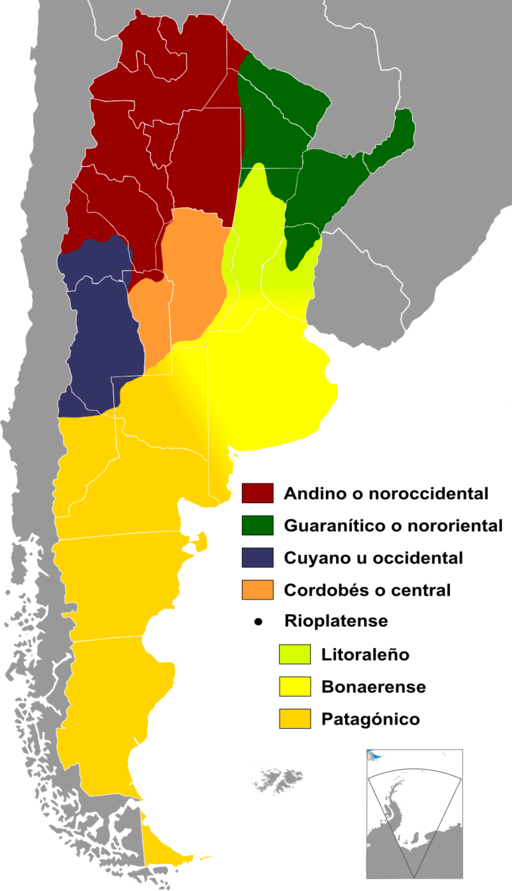
\includegraphics[width=0.5\textwidth]{Dialectos_del_idioma_espanol_en_Argentina} 
    \caption{Dialectos del idioma español en Argentina}
    \label{fig11}
\end{figure}

La motivación de esta tesis es realizar un sistema que pueda facilitar estos problemas. Vamos a enfrentar cada uno de ellos y intentar resolverlos de forma computacional. De los problemas descriptos el problema principal radica en obtener cada grabación. Si los grupos se encuentran muy alejados esto puede ser muy costoso por los viajes. También estas grabaciones deben ser de calidad aceptable como para realizar el estudio en cuestión. Se podría utilizar el teléfono para algunos experimentos pero hay que tener en cuenta que posee muy baja calidad. De hecho, se utiliza en algunos experimentos donde esta característica no afecta. 

El sistema desarrollado utiliza Internet como herramienta para obtener muestras. De esta forma, se puede realizar varias grabaciones sin necesidad de viajar a cada lugar. Es cierto que no todos los lugares poseen acceso a Internet y para lugares alejados puede ser muy contraproducente. De cualquier forma, pensamos su utilización soluciona muchos inconvenientes. Otra ventaja radica en que se puede manejar la calidad de la grabación. Utilizando distintas tecnologías a través de esta red se puede configurar la calidad para que sea lo más precisa posible para el experimento. Vamos a realizar un sistema para mejorar este proceso y diseñaremos un experimento para corroborar las ventajas y desventajas de utilizarlo. 

El experimento que tomamos como caso particular es las diferencias en el habla entre Córdoba y Buenos Aires. Estos dos grupos se encuentran uno en la zona central de nuestro país y el otro cerca del Río de la Plata, como se puede observar en la Figura \ref{fig11}. Ya se encuentran estudios que explican estas diferencias. Algunos de ellos son: \textit{El español en la Argentina} de Beatríz Fontanella de Weinberg  y \textit{Español en la Argentina} de Elena Vidal  

En el libro \textit{El español en la Argentina}, Beatríz Fontanella de Weinberg recompila varios trabajos de colegas donde analizan el español de cada región de Argentina. Cada región tiene un capítulo y entre ellas se encuentra una para Buenos Aires y otra para Córdoba. En la descripción de estos capítulos hace hincapié en los sonidos más suaves y cortos de la /r/ y /y/ y en la aspiración de la /s/. También afirma el estiramiento de la sílaba anterior a la acentuada en cada palabra como distintivo del acento. En el libro \textit{Español en la Argentina}, Elena Vidal analiza región por región el uso de los fonemas importantes. Destaca la diferencia entre las dos regiones de la /r/, /s/ y de la /ll/. También referencia a la pronunciación de la /s/.
%pagina 85 Fontanella 

Extrayendo el análisis de estos libros pude definir las reglas que describen a cada grupo. Las reglas son: 

%%\section*{Diferencias entre hablantes}
\subsection*{Regla 1: Para hablantes de Córdoba, localice la sílaba acentuada en la palabra y estirar la silaba anterior. En Buenos Aires no realizan esto. }

Cada palabra posee su sílaba acentuada. Para cumplir esta regla se debe estirar la sílaba anterior a esta. Si la sílaba acentuada es la primera de la palabra, entonces no se estira. 

Ejemplo: 'Espectacular' posee su sílaba acentuada en '-lar'. La sílaba anterior, o sea '-cu-' se alarga. 

%%De la regla 1: Se estira en la vocal. 

\subsection*{Regla 2: Para hablantes de Córdoba aspiración y elisión de /s/ al finalizar una palabra. No para Buenos Aires}

Para las palabras terminadas en /s/ se debe acortar su duración para Córdoba. 

Ejemplo: 'Pájaros' posee el fonema /s/ al final. Utilizando la dialéctica de Córdoba, la /s/ final sería mas suave que una de Buenos Aires. 

\subsection*{Regla 3: Para hablantes de Córdoba, la /s/ antes de la /c/ o /t/ suenan suaves. Para hablantes de Buenos Aires suenan sin ninguna particularidad}

La sílaba /s/, que precede a /c/ o /t/, debe sonar suave. 

Ejemplo: 'Mosca' en el dialéctico de Córdoba posee una sílaba más suave en el fonema /s/ que en Buenos Aires. 

\subsection*{Regla 4: La 'c' antes de la 't' no se pronuncia para hablantes de Córdoba. No para Buenos Aires}

La sílaba /c/, que precede a /t/, no se debe pronunciar. 

Ejemplo: 'Doctor' no debe sonar el fonema /c/.

\subsection*{Regla 5: Para hablantes Cordobeces la ‘y’ y ‘ll’ se pasa a ‘i’. No sucede esto en Buenos Aires}

Palabras con el fonema /y/ o /ll/ se pronuncian /i/. 

Ejemplo: 'lluvia' se debe pronunciar utilizando el fonema /i/ 

\subsection*{Regla 6: En hablantes Cordobeces la /r/ no debe sonar. No debe vibrar. Lo contrario para en Buenos Aires}

Palabras con el fonema /r/ deben ser suaves y no vibrar. 

Ejemplo: 'Espárrago' debe ser suave en comparación de Buenos Aires. 

Cabe destacar que estas reglas se producen en habla espontánea. No surgen de habla leída. Algunas pueden agudizarse si se encuentran en lugares económicamente más vulnerables. Pero en cualquier ambiente se cumple.

Vamos a diseñar el experimento para obtener muestras en este caso.

\chapter{Diseño del experimento}

%Utilizando estas reglas voy a definir varias actividades donde se tratará de extraer estas diferencias de la mejor forma posible. También hablaremos de las dificultades encontradas y como mejorarlo mediante trabajos futuros. Por último, mostraré si las diferencias pueden ser apreciables con el conjunto de datos extraído.

Utilizando estudios previos de ambos dialectos, pude extraer dichas reglas que describen la diferencia entre cada uno de los dos grupos. Vamos a proponer realizar un experimento para poder extraer la información fonética de los mismos. El experimento va a poner foco primordialmente en las diferencias antes descriptas. La idea sera realizar una serie de actividades donde el hablante sea grabado y esas actividades hagan hincapié en las diferencias. A continuación vamos a describir el experimento en más detalle.

%\section{Motivación}
%\paragraph{Actividades}

%Pensándolo más en detalle, nos quedamos con leer una frase. Descartamos leer una palabra porque no lograba darle una entonación interesante. Descartamos describir una imagen ya que las descripciones añaden cierta ambigüedad que hace que las palabras usadas no sean las apropiadas para identificar las diferencias de cada acento.

%Descartamos decir una palabra y decir una imagen por los siguientes motivos. Sobre decir una palabra: uno de los principales objetivos es extraer la espontaneidad del hablante. Realmente si uno dice una palabra no le impregna espontaneidad ya que es una palabra sola y leída. Sobre la imagen: si bien posee mucha espontaneidad puede suceder que la variabilidad sea muy grande. Varios hablantes podrían decir cosas completamente distintas y no podríamos obtener ninguna de las reglas propuestas.

\subsection{Frases conocidas}

Como el acento se potencia cuando se realiza habla espontánea, vamos a querer que el hablante lo diga de forma lo más natural posible. Es por ello que se nos ocurrió como actividad pronunciar frases popularmente conocidas. Pensé que si el hablante conoce la frase y es frecuente de pronunciarla, es más fácil obtener habla espontánea.

Vamos a querer utilizar frases lo mas conocidas posibles, para que el hablante ya tenga registrada como decirla sin poderle eliminar el acento.

\section{Diseño teórico}

Para realizar las grabaciones debemos darle a cada hablante una serie de frases a grabar. A esa serie de frases las llamaremos trazas.

\paragraph{Descripción de los 2 tipos de frases}
%-Descripción de los 2 grupos. Porque cada uno. Espontaneidad vs Regla 1

Vamos a tener dos formas de grabaciones: frases comunes que tratan de cubrir la espontaneidad (cubriendo las reglas 2 al 5) y frases AMPER que tratan de cubrir el acento barriendo por cada tipo de acentuación (regla 1). A continuación vemos las reglas en sus dos conjuntos.

\subsection{Frases utilizadas}

\begin{figure}[h!]
    \centerline{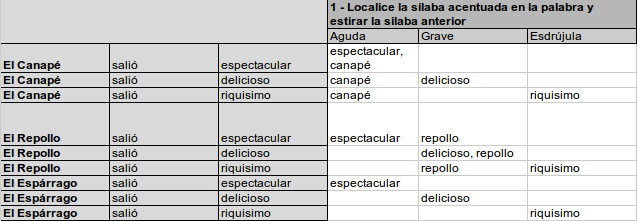
\includegraphics[width=1\textwidth]{reglas_AMPER} }
    \caption{Frases AMPER}
    \label{fig21}
\end{figure}

\begin{figure}[h!]
    \centerline{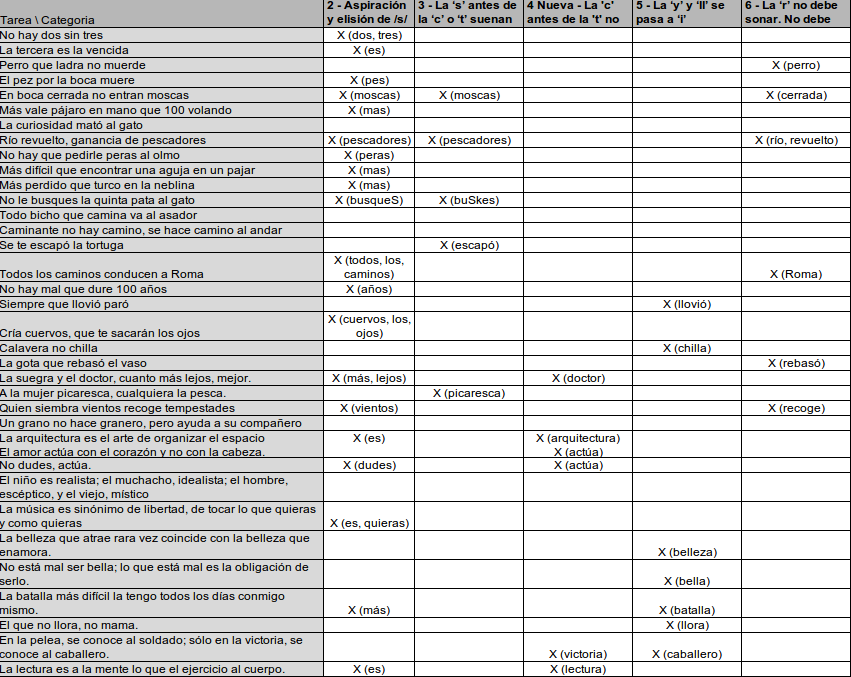
\includegraphics[width=1\textwidth]{frases_inf} }
    \caption{Frases conocidas}
    \label{fig22}
\end{figure}

\subsection{Utilizar AMPER}

%AMPER-ARGENTINA: VARIABILIDAD RÍTMICA EN DOS CORPUS 
%Jorge A. Gurlekian LIS - Conicet y UBA jag@fmed.uba.ar 
%Reina Yanagida LIS y Universidad Municipal de Estudios Extranjeros de Kobe, Japón reinay@hotmail.co.jp 
%Mónica Noemí Trípodi LIS – UBA monica906@hotmail.com 
%Guillermo Toledo Conicet y Universidad Laval, Canadá guillermo.toledo@sympatico.ca 

Utilizamos este esquema para analizar todas las variantes posibles de la Regla 1. Recordemos que la regla 1 nos dice que hay que estirar la sílaba anterior a la acentuada. Esta regla es la más conocida y puede aparecer de varias formas. Es por eso que este esquema nos va a resultar muy útil. 

Para el esquema AMPER se fija un patrón de estructura de frases y se va cambiando las palabras que utiliza. 
El esquema AMPER utilizado es: 
\begin{center}
\textit{Objeto+” salió “+Adjetivo} 
\end{center}
donde Objeto puede ser \textit{Canapé. Repollo, Espárrago}. Adjetivo puede ser \textit{espectacular, delicioso, riquísimo}. Utilizamos estas palabras ya que cubren por la acentuación de cada tipo de palabra, o sea pasa por agudas grave y esdrújula. 

Por ejemplo: \textit{El canapé salio delicioso}. Canapé tiene acento en la última sílaba. Es una palabra aguda. Mientras que delicioso es grave. En este ejemplo podemos analizar la sílaba anterior a la acentuada de estos dos grupos. Es importante armar la mayoría de las combinaciones para obtener muchas variantes de donde se encuentra el acento. De esta forma poder obtener muchísimas variantes con respecto a la Regla 1, que nos decía estirar la sílaba anterior a la acentuada. Todas las combinaciones se pueden ver en la Figura \ref{fig21}.

%También se agregó “El rábano salió horrible” que posee un acento en la primer sílaba.

\subsection{Utilizar frases conocidas}

Como afirmamos antes, utilizo frases comunes para poder obtener los acentos de cada grupo de forma natural. Se penso que si se graba una frase popular, el hablante al estar acostumbrado a decirla no iba a poder evitar impregnarle el su acento. Todas las frases conocidas utilizadas se pueden ver en la Figura \ref{fig22}.

Algo interesante es que una misma frase puede extraer atributos para varias reglas. Por ejemplo: la frase \textit{En la pelea se conoce al soldado, sólo en la victoria se conoce al caballero} extrae atributos para las reglas 4 y 5. La palabra \textit{victoria} posee atributo para la regla 4 que nos propone medir la duración de la \textit{c} antes de la \textit{t}. Sucede igual con la palabra \textit{caballero} para la regla 5. Esta nos dice medir la duración de la \textit{ll}. De esta forma cada frase extrae los atributos lo mas posible. En la Figura (todo) podemos ver el desbalance entr la cantidad de frases utilizadas con respecto a sus reglas aplicadas. Más adelante veremos como impacta esto en las frases que vamos a pedir para grabar.

\paragraph{Intercalando los dos tipos:}

Ahora debemos intercalar las trazas de frases comunes con las frases de AMPER. Vamos a agregar 4 o 5 frases de la traza de frases comunes, luego agregar 1 o 2 frases del esquema de AMPER y así sucesivamente. La idea es no cansar al hablante con frases repetitivas y evitar que sepa de antemano que frase va a tener que grabar.

\paragraph{Siempre cada 5 grabaciones:}
La mínima cantidad de grabaciones que puede realizar un hablante son 5 grabaciones. Luego se le pregunta si quiere continuar grabando. Si acepta, se le agregan otras 5 grabaciones así sucesivamente hasta llegar a las 40 que es el total de grabaciones.

\section{Generación de trazas}

%Debemos definir qué frases y en que órden se debe decir durante el experimento. Este orden va a tener la condición de que en cada nueva frase agregada vamos a querer cubrir lo mayor posible el porcentaje de cubrimiento de cada una de las reglas. Utilizaremos un algoritmo goloso para generar la traza hasta poder cubrir el 100\% de cada regla.

%La idea del algoritmo para generar trazas se va a basar en utilizar la frase que mayor información aporte en cada paso. No es lo mismo grabar una frase que solo aporta información a la regla 2 que una que aporta a la regla 2, 3, 4. Por ello, en cada paso se va agregando una frase que no fue utilizada y además que aporte la mayor cantidad de información. Es importante aplicar esta idea ya que no sabemos cuanto tiempo va a querer/tener un hablante para realizar el experimento. Utilizando nuestro algoritmo, podemos afirmar que ya con 10 frases grabadas se cubre con todas las reglas propuestas anteriormente. En el gráfico podemos ver el desempeño de nuetro algoritmo. 

Debemos definir qué frases y en que orden se debe decir durante el experimento. Sucede que el orden que utilicemos va a ser crucial para tener muestras. No es lo mismo empezar por una frase que sólo referencia a una regla que a varias. Si referencia a varias reglas a la vez, en un sólo audio podremos sacarle más información.

Una traza es una lista de las frases que puede grabar un hablante. Un hablante al empezar se le dará una de estas y grabará sucesivamente en ese orden. Optamos por tener precalculada las trazas para evitar cálculos innecesarios a la hora de empezar el experimento. Es por eso que guardamos 10.000 trazas generadas. 

La generación de trazas sigue el siguiente algoritmo:

\lstset{ %
language=C++,                % choose the language of the code
basicstyle=\footnotesize,       % the size of the fonts that are used for the code
numbers=left,                   % where to put the line-numbers
numberstyle=\footnotesize,      % the size of the fonts that are used for the line-numbers
stepnumber=1,                   % the step between two line-numbers. If it is 1 each line will be numbered
numbersep=5pt,                  % how far the line-numbers are from the code
backgroundcolor=\color{white},  % choose the background color. You must add \usepackage{color}
showspaces=false,               % show spaces adding particular underscores
showstringspaces=false,         % underline spaces within strings
showtabs=false,                 % show tabs within strings adding particular underscores
frame=single,           % adds a frame around the code
tabsize=2,          % sets default tabsize to 2 spaces
captionpos=b,           % sets the caption-position to bottom
breaklines=true,        % sets automatic line breaking
breakatwhitespace=false,    % sets if automatic breaks should only happen at whitespace
escapeinside={\%*}{*)}          % if you want to add a comment within your code
}
\begin{lstlisting}
    Genrador de trazas:
    Input: Frases
    Output: listaFrases 
    listaFrases = {}
    DicPct <- Diccionario de porcentajes de cada regla
    Mientras Frases != {}:
    	regla <- Obtener regla con mejor porcentaje
    	CtoFrases <- frases.ObtenerDeLaReglaLasMasPonderadas(regla)
    	listaFrases.agregar(CtoFrases)
    	RecalcularPorcentajes(DicPct)
    Devolver listaFrases
\end{lstlisting}

La idea del algoritmo es la siguiente: Al generar las trazas vamos a utilizar un contador que nos va a decir cuantas muestras tenemos por cada regla. En cada paso vamos a ver ese contador y vamos a elegir la próxima frase teniéndolo en cuenta. Elegiremos la frase que haga referencia a la regla menos grabada en el contador y además que represente a mas de una regla. De esa forma intentamos obtener la mayor cantidad de información posible con pocas grabaciones y ponderamos las frases que referencien a más reglas. 

Esta idea es importante ya que maximizamos la cantidad de información de cada frase y al hablante le hacemos perder menos tiempo realizando el experimento. Esto se puede ver en el gráfico \ref{figFracesTraza} que representa el porcentaje de frases completadas mientras se va aumentando la cantidad de grabaciones. Teniendo en cuenta este algoritmo podemos notar que a partir de 10 grabaciones ya tenemos un buen porcentaje de cubrimiento de todas las reglas. Escluimos del gráfico la regla 1 ya que esta utiliza con las frases AMPER.

\begin{figure}[h!]
    \centerline{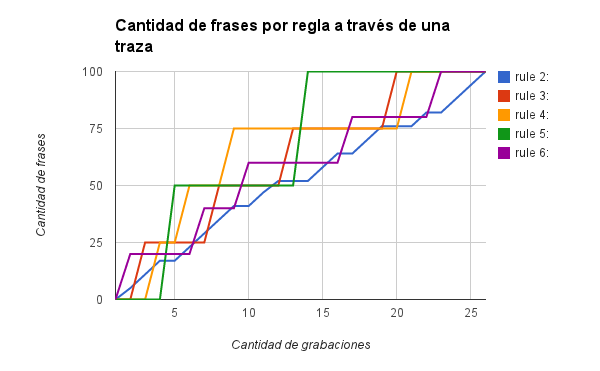
\includegraphics[width=0.9\textwidth]{cant_frases_traza_inf} }
    \caption{Cantidad de frases por traza}
    \label{figFracesTraza}
\end{figure}

En conclusión, se grabarán de a 5 frases. Teniendo en cuenta que las primeras serán frases conocídas y las últimas 2 corresponderán al esquema AMPER. 

\chapter{Sistema de grabación online}

Para poder obtener audios de distintas personas se desarrolló una página web. Esto nos da muchas ventajas ya que nos permite grabar fácilmente desde cualquier lugar. En esta sección explicaremos la arquitectura del sistema y sus detalles técnicos.

La página web esta desarrollada en Django versión 1.4.2 que es un framework para la creación de paginas web. Se eligió este framework por su facilidad a la hora de salvar objetos a la base de datos y también por la cantidad importante de librerías que posee Python. La versión utilizada de Python es 2.7.3. Esta misma necesita una base de datos para guardar cada clase de dominio. En esta base vamos a guardar los datos de cada hablante, las frases a grabar y las trazas principalmente. La base de datos utilizada fue PostgreSQL versión 9.1 y se eligió esta ya que es de código abierto. Para el servidor HTTP se utilizó Apache versión 2.2.22. El servidor corre en el sistema operativo Ubuntu 12.04.4 LTS.

\section{Recolección de datos}

Cuando un usuario visita nuestra página, primero le hace llenar un formulario. Este le pregunta: género, fecha de nacimiento y de qué lugar es oriundo. Al confirmar los datos, estos son grabados en la base de datos de la aplicación en el servidor. Esto se puede apreciar en la Figura \ref{figEncuesta}. Luego se procede a realizar las grabaciones. 

\begin{figure}[h!]
    \centerline{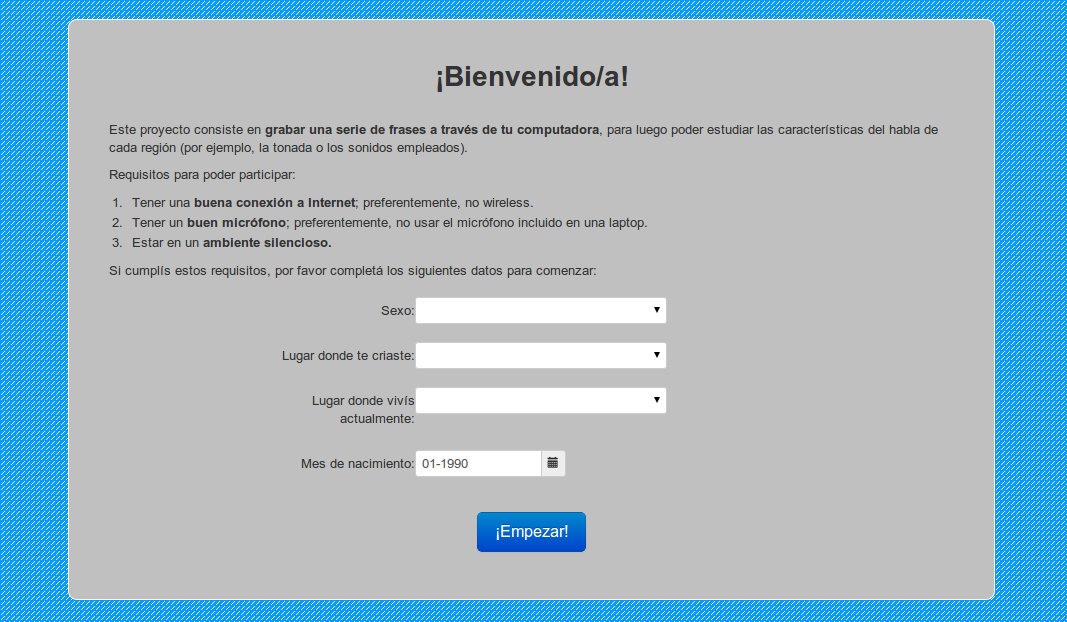
\includegraphics[width=0.7\textwidth]{pag-inicio2} }
    \caption{Encuesta}
    \label{figEncuesta}
\end{figure}

\begin{figure}[h!]
    \centerline{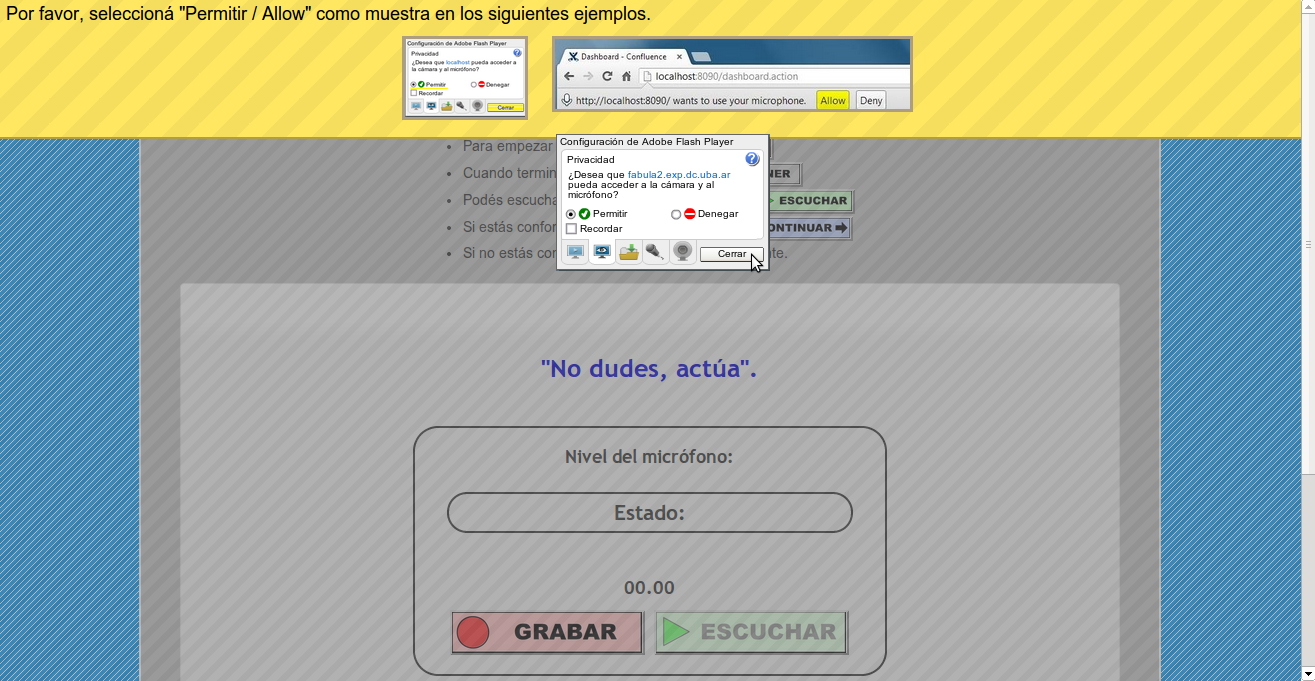
\includegraphics[width=0.7\textwidth]{pag-allow1} }
    \caption{Permitir micrófono}
    \label{allowmic}
\end{figure}

\begin{figure}[h!]
    \centerline{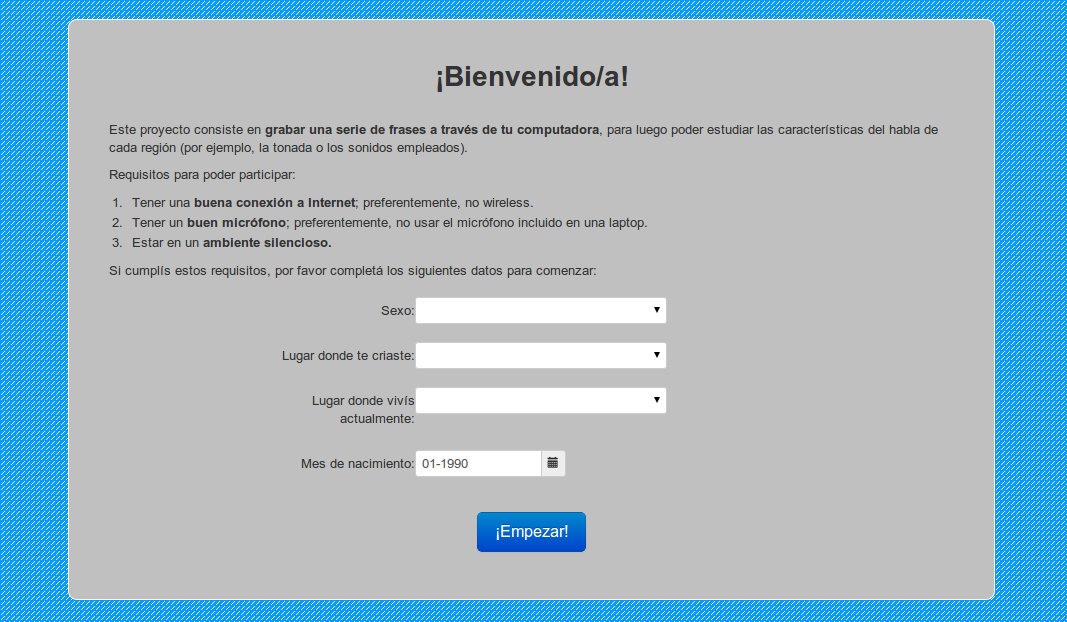
\includegraphics[width=0.7\textwidth]{pag-inicio2} }
    \caption{Inicio}
    \label{inicio}
\end{figure}

\begin{figure}[h!]
    \centerline{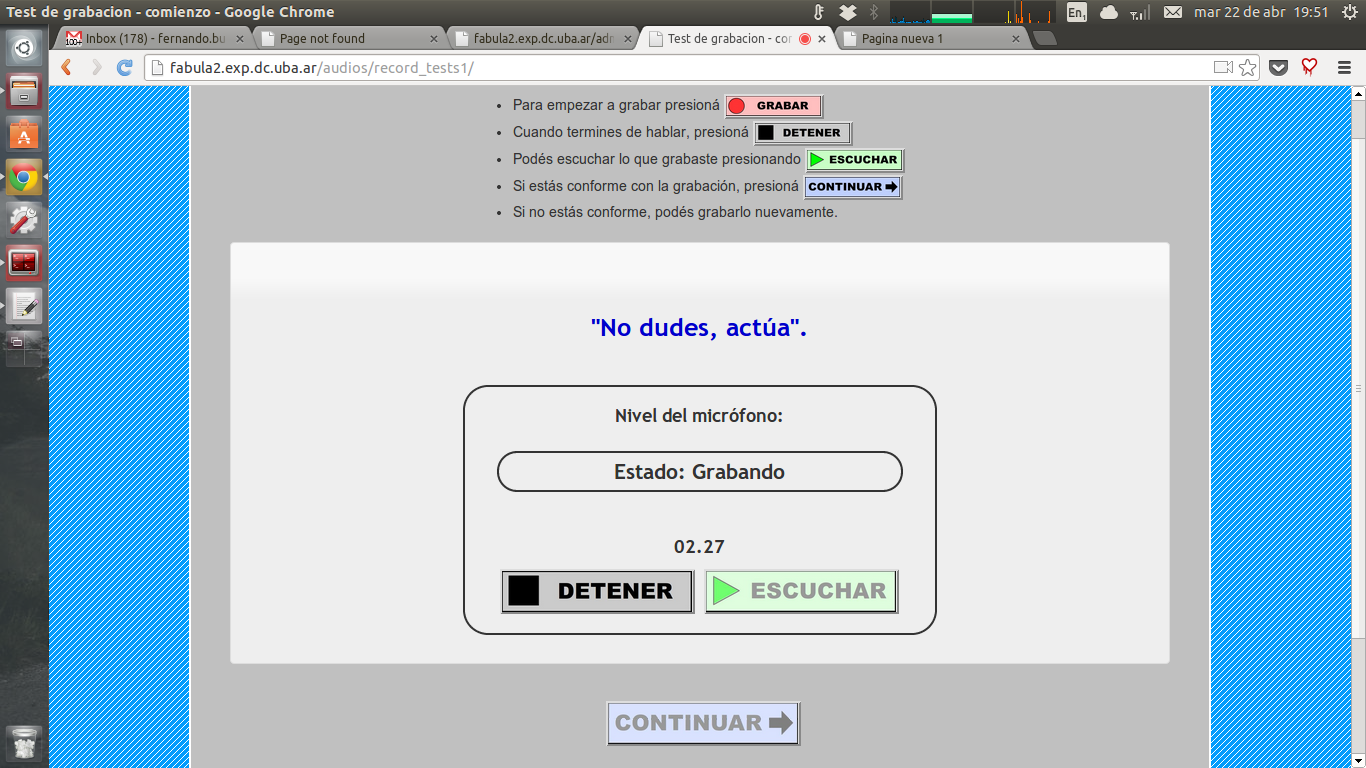
\includegraphics[width=0.7\textwidth]{pag-grabar1} }
    \caption{Grabando}
    \label{grabando}
\end{figure}

\begin{figure}[h!]
    \centerline{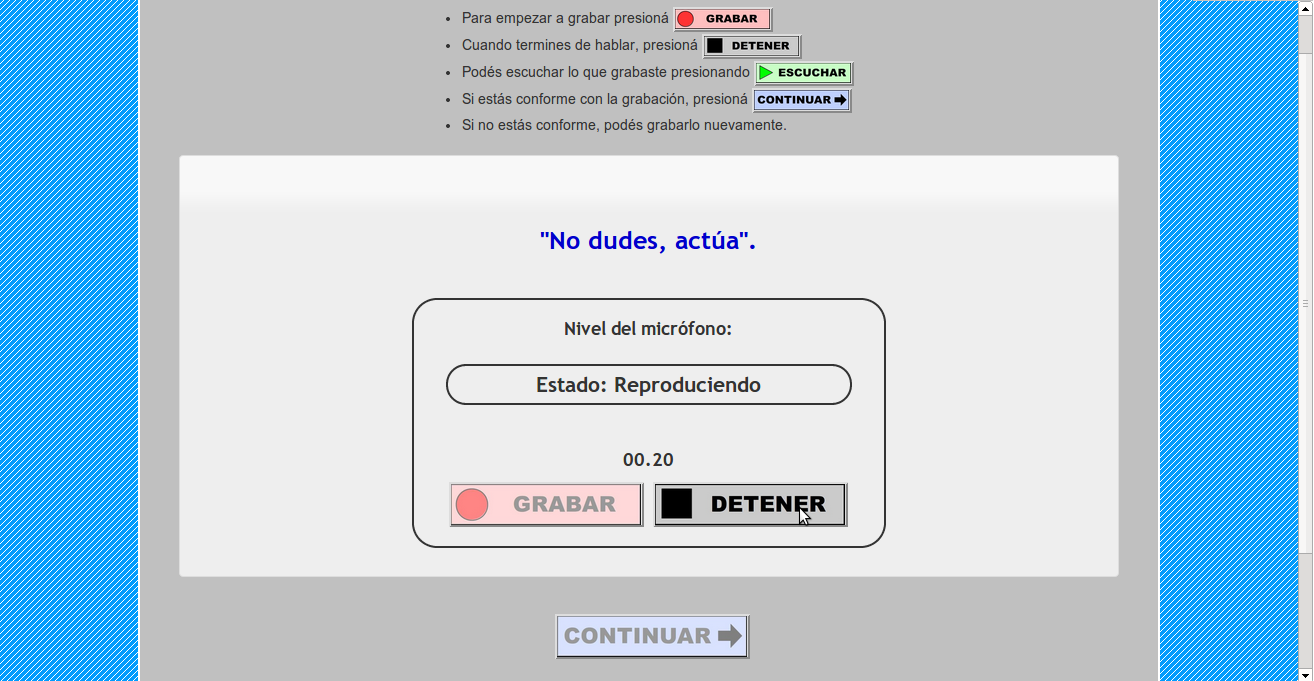
\includegraphics[width=0.7\textwidth]{pag-play1} }
    \caption{Reproduciendo}
    \label{reproduciendo}
\end{figure}

En la pantalla de grabación el usuario deberá confirmar tener acceso al micrófono que posee en su dispositivo, como se puede ver en la Figura \ref{allowmic}.  Una vez hecho esto, se le explica las instrucciones (Fig. \ref{inicio}) y puede empezar a grabar. Cada nuevo experimento utiliza una nueva traza. El experimento en total consiste en realizar 40 grabaciones. El hablante va grabando de a 5 frases, cada vez que las termina de grabar ofrece la opción de seguir grabando otras 5 más. De esta forma, aporta el tiempo que puede. La interfaz de como se ve cuando el usuario graba se puede ver en la Figura \ref{grabando}. Las grabaciones pueden ser escuchadas antes de ser confirmadas por el usuario. Lo importante es que la grabación se escuchen lo mejor posible. Para reproducir se aprieta en el botón \textit{Reproducir} como se ve en Figura \ref{reproduciendo}.

Cada vez que se confirma una grabación, esta se graba en un archivo wav en el servidor. 

%todo: PONER DATOS TECNICOS DEL TIPO DE WAV

\section{Grabación a través del browser}

Los navegadores actuales no pueden soportar acceder al micrófono directamente. Durante la tesis, se desarrolla HTML5 que podrá soportar acceder al micrófono más fácil. No se eligió basarse en este porque sólo algunos browsers lo soportaban y al ser un estándar muy nuevo necesita que el usuario tenga instalada últimas versiones de software y eso excluiría gente. Es por eso que debimos utilizar alguna tecnología alternativa. Buscando encontré un proyecto llamado WAMI que es una aplicación Flash que nos permite acceder al micrófono a través de JavaScript. 

El proyecto WAMI (http://code.google.com/p/wami-recorder/) nos permite acceder al micrófono de la computadora utilizando Flash. Este posee una interfaz que permite utilizar la aplicación Flash desde Javascript. De esta forma, no es necesario meterse en la implementación. Utilizando dicha interfaz se puede configurar varias urls. Una de ellas es donde envía la información de lo grabado.

Cuando termina de grabar, se envía un mensaje POST al servidor. Este obtiene el paquete de información y lo guarda como archivo .wav. Cuando se quiere reproducir algún audio se envía un mensaje GET a través de la interfaz. El servidor lo responde con el audio requerido y se reproduce en el navegador. 

Como se mencionó antes, para poder acceder al micrófono el usuario debe habilitar permisos para que la aplicación acceda al hardware de su computadora. Esto aparece como una ventana emergente al principio del experimento. Esto se puede ver en la Figura \ref{allowmic}. También se puede configurar la calidad del audio grabado y analizar el nivel del volumen que posee. Se guarda un registro de nivel de volumen sobre la interfaz para utilizar esos datos en algún proyecto futuro.

\section{Requerimientos}

Los requerimientos son básicos: micrófono, conexión a internet. 
Tuvimos problemas sobre el browser que utilizaba. Wami necesita Flash versión 11.04 (chequear) que no se encuentra en los repositorios tradicionales de Ubuntu. De esta manera, los navegadores que utilicen Flash instalado por el sistema operativo Ubuntu no podrán correr. Otros sistemas operativos, como Windows o IOs, no tienen problemas en la versión de Flash instalada. De todas formas el navegador Chrome posee preinstalado dicha versión de Flash, entonces este navegador podía correr perfectamente la aplicación sin importar el sistema operativo.

\section{Sistema de administración}

El sistema debe tener datos cargados para estan online recolectando audios. Los minimos datos para poder tener la página funcionando en vivo son los datos de las trazas y la clasificación de los audios. Este cargo de datos se pueden guardar con fixtures del framework Django. Una vez cargado esos datos, los hablantes van a acceder a una url donde van a poder realizar el experimento grabando los distintos audios.

\subsection{Etiquetando audios}

Cuando varias personas terminan el experimento, los administradores pueden acceder a una url donde se puede escuchar cada audio que se va generando. Y si fue exitoso, o sea no esta saturado y no tiene ruidos, puede etiquetarlo con alguna de las etiquetas definidas. Las etiquetadas utilizadas esta vez son: ‘Conservar’,  ‘Sonido saturado’, ‘Mucho ruido de fondo’, ‘Problemas en el habla’. Más adelante veremos como obtener estos audios. Esto se puede ver en Figura \ref{cat}.

\begin{figure}[h!]
    \centerline{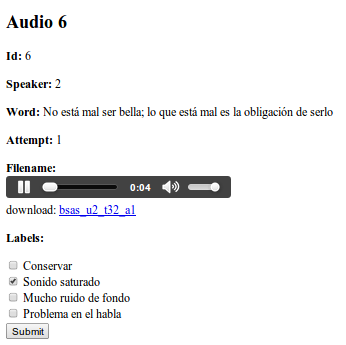
\includegraphics[width=0.5\textwidth]{categorizando_audios} }
    \caption{Categorizando audios}
    \label{cat}
\end{figure}

\paragraph{Backups automáticos}

El sistema posee backups automáticos generados a la noche automáticamente. Los backups consisten en un dump de la base de datos y de sincronizacion de los audios con una carpeta de backup. De esta forma, se guardan todos los datos cada día, y los audios quedan a salvo.

\paragraph{Export de wavs y csv}

Luego de obtener varios audios podemos exportar todos los datos a traves de urls. Utilizamos distintas urls que nos van a permitir bajarnos los audios etiquetados. Por ejemplo si accedemos a /conservados vamos a bajar los audios etiquetados de esa forma. Idem para las demas. Tambien se pueden bajar todos los audios sin etiquetas. Sobre la base de datos, se pueden bajar todo el modelo de datos a formato csv.

\section{Filtrado de audios}

Debemos evitar grabar audios saturados. Para ello se nos ocurrió medir el volumen de la grabación cuando sucede la misma. El resultado es una serie de valores entre 0 a 100. Sobre estos valores vamos a calcular el máximo y el mínimo. Si el primero es mayor a un cierto umbral (o sea mayor a 80) quiere decir que en la grabación se saturó en algún momento. Si el mínimo es menor a un cierto umbral (o sea menor a 20 por ejemplo) quiere decir que hay mucho sonido ambiente. En cualquiera de los dos casos podemos pedirle al usuario que grabe devuelta el experimento. De esta forma podemos filtar audios que no nos servirán para reconocer el acento.

Si bien esta característica esta fue programada, no fue utilizada en la recolección de datos. El motivo fue que queríamos chequear cuan bien funcionaba la herramienta sin filtros y con completa participación de los usuarios. Otro motivo fue la paciencia de los hablantes. Puede suceder que al tratar de grabar no logre un ambiente beneficioso para grabar. Esto quiere decir que aunque quiera grabar el filtro rechace todos sus audios. También notamos que había grabaciones que dieron mal el filtrado del volumen pero la grabación era buena. Esto no lo queremos como primer experimento del framework. Por eso optamos por aceptar todos sus audios.

Para los audios que salieron saturados, más adelante vamos a realizar un estudio para intentar sacarles el ruido y de esta forma intentar rescatarlos.

\section{Varias grabaciones por frase}

Siguiendo con la idea de tener la mejor grabación de cada hablante, le dimos la opción a cada hablante de que después de grabar un audio de una frase puedan escucharse como quedó. Esto requiere un ida y vuelta entre el cliente (navegador) y el servidor. Al grabar, el cliente manda un mensaje HTTP POST para el servidor con los datos de grabación. Las frases son cortas entonces no es necesario preocuparse por la longitud del paquete. Cuando el cliente quiere escucharlo envía un mensaje GET a ese mismo audio anteriormente grabado. El servidor envía la grabación y es reproducida en el cliente. Esta ida y vuelta de la grabación podría ser optimizada para que la grabación pueda ser escuchada sin tener interacción con el servidor. En nuestro experimento, no tuvimos problemas graves en lo que respecta a latencias pero si es un punto débil del sistema.

A cada hablante le dimos la opción que pueda escuchar y volver a grabar la frase cuantas veces quisiera. Esto lo hicimos para poder detectar cual es el disparador que hace que diga mal una frase. Puede resultar interesante analizar los anteriores audios y porque se queda con el último.

\chapter{Extracción de información}

Utilizando nuestra página web se van a poder obtener distintas muestras de Córdoba y Buenos Aires. Pero ¿Cómo podemos analizar estos audios correctamente?. Un archivo wav, como los que captura la página cada una de las pruebas, posee muchísima información. Es por esto que debemos seleccionar correctamente que partes de la información nos sirve y que partes podemos descartar. 

\section{Alineación forzada}

Un dato muy importante es que esta selección idealmente no debe tener que ser realizada con intervención de un humano. Ya que, si tenemos muchos audios tendríamos que hacerlo uno por uno y sería un trabajo muy arduo. De esto se encarga la alineación forzada. Las partes que debemos extraer de los audios son las partes donde se encuentran la diferencias de cada regla descripta anteriormente. Debemos tener una herramienta que nos permita obtener esas pequeños pedazos de audios para analizar sus diferencias. 

\subsection{Prosodylab Aligner}

%If you use this tool, we would appreciate it if you cite the following paper:
%Gorman, Kyle, Jonathan Howell & Michael Wagner (2011). Prosodylab-Aligner: A tool for forced alignment of laboratory speech. Proceedings of Acoustics Week in Canada, Quebec City.

Luego de buscar bastantes, encontramos con una herramienta llamada ProsodyLab Aligner \cite{prosodylab}. Su función es realizar alineaciones automáticas en cada uno de los audios de forma fácil. O sea, va analizar cada audio y mediante un diccionario determina cada fonema en que momento se dijo. El formato utilizado para devolver estas marcas es el TextGrid. El problema de la alineación es un sub-problema de la alineación automática.

Algo que destaca esta herramienta es que no necesita datos de entrenamiento. Sólo con una hora de grabación es suficiente para correrlo y obtener resultados. Otra ventaja es que puede utilizarse para cualquier idioma. 

%implementación
Esta herramienta esta hecha íntegramente en lenguaje Python (ver. 2.5) y script de Linux. Utiliza fuertemente de HTK (ver. 3.4) y SoX (ver. 14.1.0). Para realizar la alineación utiliza Modelos Ocultos de Markov \cite{rabiner} (en ingles HMM). Básicamente trata de predecir que fonemas aparecen en cada parte del los audios utilizando las diferentes muestras y la lista de fonemas pronunciada en cada grabación. Por ejemplo: mediante un modelo matemático el programa analiza que en muchas grabaciones de la misma frase se produce un mismo fonema. Ese fonema va a ser marcado de igual forma en el TextGrid de las tres grabaciones.

%Una de las ventajas que posee es que puede utilizarse para cualquier idioma. Sólo se necesita una hora de audio grabado y un diccionario fonético sobre las palabras a reconocer. 

La hora de grabación la debíamos cumplir recolectando grabaciones de la página web. Esta meta era posible de realizar. La creación de un diccionario era más complicado, ya que debía ser en español. Gracias a Laboratorio de Investigaciones Sensoriales - INIGEM que nos prestó su diccionario pudimos utilizar esta herramienta. El diccionario fonético nos provee para cada palabra los distintos fonemas que la componen. Esta herramienta se utiliza para generar la lista de fonemas que aparecen en cada grabación. De esta manera, se puede realizar una alineación acorde al español.

\subsection{Diccionario TranscriptorFonetico2 del LIS}

Un diccionario fonético es básicamente un listado con las palabras que utilizamos y su división en fonemas. Es importante esto ya que va a ser usado por el alineador para describir los fonemas de cada palabra para cada grabación.

\section{Extracción de atributos}

En esta sección vamos a analizar como extraer cada uno de los atributos que planteamos en cada regla.

\subsection{Implementación}

La extracción de datos fue realizado utilizando el lenguaje Python. Elegimos ese ya que es un lenguaje de fácil de programar y tiene muchas librerías útiles para este tipo de casos. Utilizamos una muy conocida llamada Numpy versión 1.6.1. Esta es una librería para el calculo preciso en aplicaciones científicas.

El extractor posee como input los archivos .wav y los archivos textgrid que corresponden a las alineaciones temporales de cada fonema en cada audio. El extractor se debe ejecutar después de la alineación realizada por Prosodylab Aligner. El workflow del extractor se puede ver en \ref{workflow}). 

\begin{figure}[h!]
    \centerline{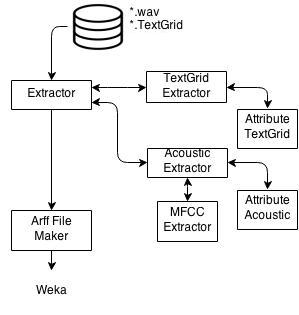
\includegraphics[width=0.5\textwidth]{diagrama_workflow} }
    \caption{Diagrama workflow}
    \label{workflow}
\end{figure}


El ProsodyLab-Algner al finalizar una alineación nos devuelve un archivo donde se encuentra como fueron realizadas esas alineaciones. Este archivo se llama '.SCORES' y en el se encuentra una lista de todos los audios seguidos de un valor. Este valor nos permite ver la verosimilitud de las alineaciones. Si una alineación fue similar a otra va a tener aproximadamente un valor similar. En cambio, si posee una alineación muy distinta va a tener valores muy distintos. Este va a ser el primer filtro para el extractor. Ordenando los audios en esta escala notamos que los menores poseen alineaciones malas, entonces definimos un umbral para el cual aceptar y rechazar la alineación. Si bien este procedimiento es efectivo, notamos que se encuentran algunos falsos positivos, o sea archivos que tienen un buen punto de score pero la alineación es mala. Al tener pocas grabaciones no pudimos aceptar estos casos, debimos corregirlos.

Luego de esto, el extractor va a correr un conjunto de funciones que van a extraer cada uno de los atributos. Este conjunto de funciones se dividen en dos: las que computan atributos temporales y las que computan atributos acústicos. Veamos cada uno:

\subsection{Atributos temporales}

Corresponden a los atributos de duración en los fonemas y la sílabas de cada frase. Para calcularlos utilizamos como input el textgrid generado en la alineación. Básicamente estas funciones recorren el textgrid buscando un patrón en particular y lo miden.

Las mediciones son normalizadas de dos formas: primero una normalización utilizando:

\hspace{2cm} \[\frac{X - \mu }{ \sigma }\]

y luego otra asumiendo que $\mu = 0$. 

\hspace{2cm} \[\frac{X}{ \sigma }\]

Esta ultima tiene el nombre de half normal distribution.

%todo: agregar imagen explicando normalización

los atributos temporales se dividen en dos grupos: fonéticos y silábicos. Cada grupo calcula igual la normalización pero uno va a tener en cuenta fonemas y otro sílabas. Veamos cuales son:

\subsubsection{Atributos fonéticos}

\begin{itemize}
    \item \textbf{Duración de la 'kt':} con este atributo vamos a buscar el patrón 'kt' en los TextGrids y luego a medir normalizando de las dos formas el fonema 'k'.  
    \item \textbf{Duración de la 'sc':} ídem con 'sc' y midiendo el fonema 's'.
    \item \textbf{Duración de la 'll':} buscamos el patrón 'll' y lo medimos normalizandolo de las dos formas.
    \item \textbf{Duración de la 'rr':} ídem para 'rr'.
    \item \textbf{Duración de la 's' final:} Ídem para las 's' de final de palabra.
    
    \item \textbf{Duración de cada fonema:} este atributo mide la cantidad de fonemas y realiza un promedio. Este no se realiza normalización.  
    \item \textbf{Duración de cada vocal:} contabilizamos cada vocal y luego realizamos su normalización utilizando la duración de cada fonema.
    \item \textbf{Duración de cada consonante:} Ídem para consonantes. 
\end{itemize}

\subsubsection{Atributos silábicos}

Vamos a hacer un análisis de la sílabas. Los atributos que usamos son:

\begin{itemize}
    \item \textbf{Duración de la sílaba acentuada:} en cada una de las frases vamos a buscar la sílaba acentuada de cada palabra, mediremos su duración y normalizaremos con las demás sílabas.
    \item \textbf{Duración de la sílaba anterior a la acentuada:} realizamos el mismo calculo anterior pero con la sílaba previa a la acentuada. 
\end{itemize}

Estos atributos usamos para poder medir fuertemente la Regla 1, que esta es la más resaltada de la tonada cordobesa. Para saber cual es la sílaba acentuada se realizó un script que describe para cada frase cuales son sus sílabas acentuadas. Este se encuentra en el Anexo.

\subsection{Atributos acústicos}

Los atributos acústicos utilizan las propiedades de los wavs grabados. Para ello debimos extraer información con algún método que permita medirlos. Elegimos el calculo de MFCC ya que tiene relación directa con la percepción auditiva humana. 


\subsubsection{Mel Frequency Cepstral Coefficients}

%http://practicalcryptography.com/miscellaneous/machine-learning/guide-mel-frequency-cepstral-coefficients-mfccs/

La forma en que hablamos se produce por varias articulaciones. Algunas de ellas pueden ser: dientes, lengua, traquea etc. Estas articulaciones trabajan de forma tal para producir el sonido. Pero también funcionan para darle forma y aplicarle un filtro al sonido producido. Si sabemos correctamente que filtro se le aplica, podremos saber que sonido produce. La forma y el filtro asociado nos muestra donde esta la fuerza en el fonema. Este filtro es muy importante para entender la percepción humana.

Las señales de audio cambian constantemente poseen muchas variaciones. En periodos cortos de tiempo estas variaciones se reducen. Vamos a dividir todo el audio en pequeños frames para calcular en ellos los coeficientes. El tamaño de cada frame esta entre 20-40 ms. Si la variación es menor a este frame, habrá pocas pruebas para tenerla en cuenta y entonces la descartaremos.

Luego para cada frame se calcula el espectro de frecuencia. Esto se viene motivado por un órgano que se encuentra en la oreja llamado Cóclea. Este vibra de diferente forma al llegarle cada frecuencia del sonido. Al vibrar, activa nervios que representan las distintas frecuencias que escuchamos. Dividir el sonido en períodos intenta mostrar que frecuencias están activas.

El Cóclea no reconoce diferencias entre dos frecuencias muy cercanas. Esto se incrementa mientras más alejada esta esa frecuencia. Para representar esta idea se utiliza un filtrado por escala de Mel. Esta escala es una aproximación de nuestra percepción. A frecuencias menores a los 1 Khz el filtro se comporta de fórma lineal. A partir de ese valor, se comporta de forma logarítmica. 

%http://i.stack.imgur.com/YUH48.gif

\begin{figure}
    \centerline{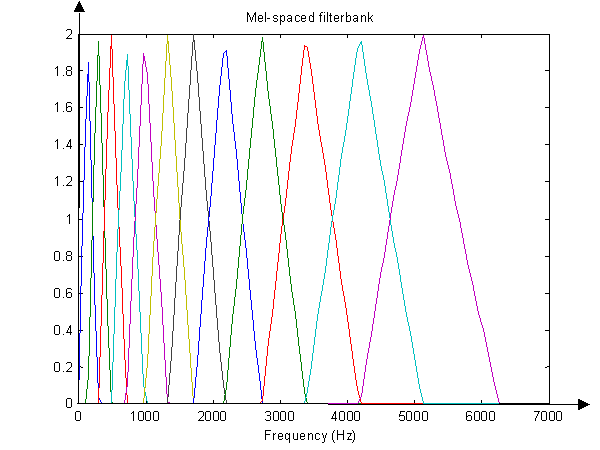
\includegraphics[width=0.5\textwidth]{mfcc} }
    \caption{Filtro MFCC}
    \label{mfcc}
\end{figure}

% todo: Aca se introduce los filtros onda serrucho. 
Mientras mas aumentamos la frecuencia, mas anchos son los filtros aplicados. Por ejemplo, ya en 4 Khz se aplican 20 filtros. (Ver Fig. \ref{mfcc}) Lo importante es ver cuanta energía hay en las frecuencias involucradas en el filtro. Luego que tenemos la energía de estos tramos le aplicamos el logaritmo. Esto se ajunta mejor a como escucha el oído. Para finalizar se computa DCT de las energías filtradas. 

El siguiente pseudocódigo explica paso a paso como se calcula los coeficientes:
\lstset{ %
language=C++,                % choose the language of the code
basicstyle=\footnotesize,       % the size of the fonts that are used for the code
numbers=left,                   % where to put the line-numbers
numberstyle=\footnotesize,      % the size of the fonts that are used for the line-numbers
stepnumber=1,                   % the step between two line-numbers. If it is 1 each line will be numbered
numbersep=5pt,                  % how far the line-numbers are from the code
backgroundcolor=\color{white},  % choose the background color. You must add \usepackage{color}
showspaces=false,               % show spaces adding particular underscores
showstringspaces=false,         % underline spaces within strings
showtabs=false,                 % show tabs within strings adding particular underscores
frame=single,           % adds a frame around the code
tabsize=2,          % sets default tabsize to 2 spaces
captionpos=b,           % sets the caption-position to bottom
breaklines=true,        % sets automatic line breaking
breakatwhitespace=false,    % sets if automatic breaks should only happen at whitespace
escapeinside={\%*}{*)}          % if you want to add a comment within your code
}
\begin{lstlisting}
MFCC (Mel frequency cepstral coefficient):
1) Aplicar la derivada de Fourier de la se\~nal. -> Espectro
2) Mapear las amplitudes del espectro a la escala mel.
3) Calcular el logaritmo.
4) Aplicar la transformada de coseno discreta (DCT).
5) Los MFCC son las amplitudes del espectro resultante.
\end{lstlisting}

Este algoritmo se calcula para un segmento del audio. El audio se debe dividir en frames de 20 o 30 milisegundos pero avanzando 10 o 15 milisegundos. Hay superposiciones en cada segmento. Al finalizar el algoritmo obtenemos 13 atributos acústicos de ese segmento. Podemos realizar la derivada de estos atributos y la segunda derivada para obtener más atributos. Estos atributos corresponden a el estiramiento de los fonemas a través del tiempo. En total derivando dos veces llegan a 33 atributos acústicos.

Debemos extraer datos de los wavs grabados. Para ello debemos analizarlos y que ese análisis nos de una medida que pueda compararse. El análisis debe tener en cuenta como lo percibe un humano. Las frecuencias de Mel ayudan a describir la percepción humana del lado de las frecuencias que escucha. 

\subsubsection{Implementación}

Para realizar el calculo de estos coeficientes se utilizó un script en Matlab. El creador del script es BLA y utiliza los 33 atributos utilizando sus primeras y segundas derivadas. El extractor necesita estos valores para cada audio a extraer. Es por eso que se conecta con Matlab a través de un wrapper para calcular el script y luego continuar con la extracción.

\chapter{Datos obtenidos}

Los audios recolectados tuvieron algunos problemas al grabarse. El principal problema fue que el ambiente que utilizó cada hablante no estaba completamente en silencio como para hacer una buena grabación. Muchos errores surgieron en esa dirección. Otros errores comunes pero no tan frecuentes fueron: interpretaciones erróneas de la consigna, errores de volumen del micrófono, saturación etc.. 

\subsection{Mediciones}

Escuché los audios para determinar si se realizaron correctamente. Los fuimos clasificando en: Conservar, Sonido saturado, Mucho ruido de fondo, Problema en el habla. Esta clasificación fue empírica, o sea no realizando ningún análisis sino que escuchando manualmente cada una. La cantidad de cada clase fue la siguiente:

\begin{table}[h]
\centering
\begin{tabular}{|l|c|c|c|c|}
\hline
\textbf{}  & \textbf{Bs.As. } & \textbf{Cba.} & \textbf{Total} \\ \hline
\textbf{Conservar}  & 222 & 105 & 327 \\ \hline
\textbf{Problemas en el habla}  & 33 & 15 & 48 \\ \hline
\textbf{Mucho ruido de fondo}  & 2 & 12 & 14 \\ \hline
\textbf{Sonido saturado}  & 2 & 0 & 2 \\ \hline
\end{tabular}
\end{table}

Algo importante de ver es que los datos obtenidos están desbalanceados. No pudimos obtener la misma cantidad de audios para los dos grupos. Esto se va a reflejar en la clasificación y en el análisis posterior.

\subsection{Errores comunes}

Las categorías establecidas anteriormente describen los errores comunes mas frecuentes. Podemos observar que del total de 391 grabaciones, 64 tuvo algún problema. Este es alrededor del 16\% de los audios grabados. Es un número alto para ser un experimento guiado. 

La gran causa de este número es la faltante de un chequeo en el mismo momento que va grabando cada uno de los audios. Un trabajo futuro sería analizar el audio grabado y rechazarlo si no supera un nivel aceptable auditivo. Esto puede implementarse de varias formas. Una posible sería cuando esta grabando medir el volumen del micrófono cada una cierta cantidad de tiempo, por ejemplo 1 segundo. Si en esa medición el volumen no se encuentra entre rango máximo y mínimo de volumen, descartar el audio y pedirle al hablante que vuelva a grabar.

%todo: esto nose si va mejor en Trabajos Futuros
También se le podría dar mas información al hablante. Sabiendo que el micrófono tuvo un pico de volumen se podría pedirle al hablante que no hable tan fuerte. Ídem si habla muy bajo. Otras posibles soluciones a este problema es analizar antes de empezar el experimento si el sonido ambiente es muy alto o no. Y luego de ello aceptar una grabación nueva. Todas esas soluciones e pueden realizar en la aplicación web sin intervenir en el servidor.

Para análisis mas precisos se puede aplicar mejores filtros cuando llega la grabación del lado del servidor. Cuando llega el mensaje del audio al servidor, este ya puede obtener el wav y realizarle todo tipo de análisis mas precisos. Recordemos que el servidor esta implementado en Python que posee muchas librerías útiles para el análisis de audios. Al momento de terminar el análisis del audio en cuestión, deberá enviar la respuesta al hablante informándole si se debe realizar devuelta la grabación o si fue exitosa. Es importante notar que esta solución necesita buena conexión para el server. 

Vamos a continuar con el análisis basándonos en los audios clasificados como Conservados. Luego trataremos de realizar algún análisis para reutilizar algunos de estos que tuvieron algún problema. 

\section{Alineación forzada}

El alineador automático no realiza su función de forma perfecta. Sucede que muchas veces alinea mal. 

\begin{figure}[h!]
    \centerline{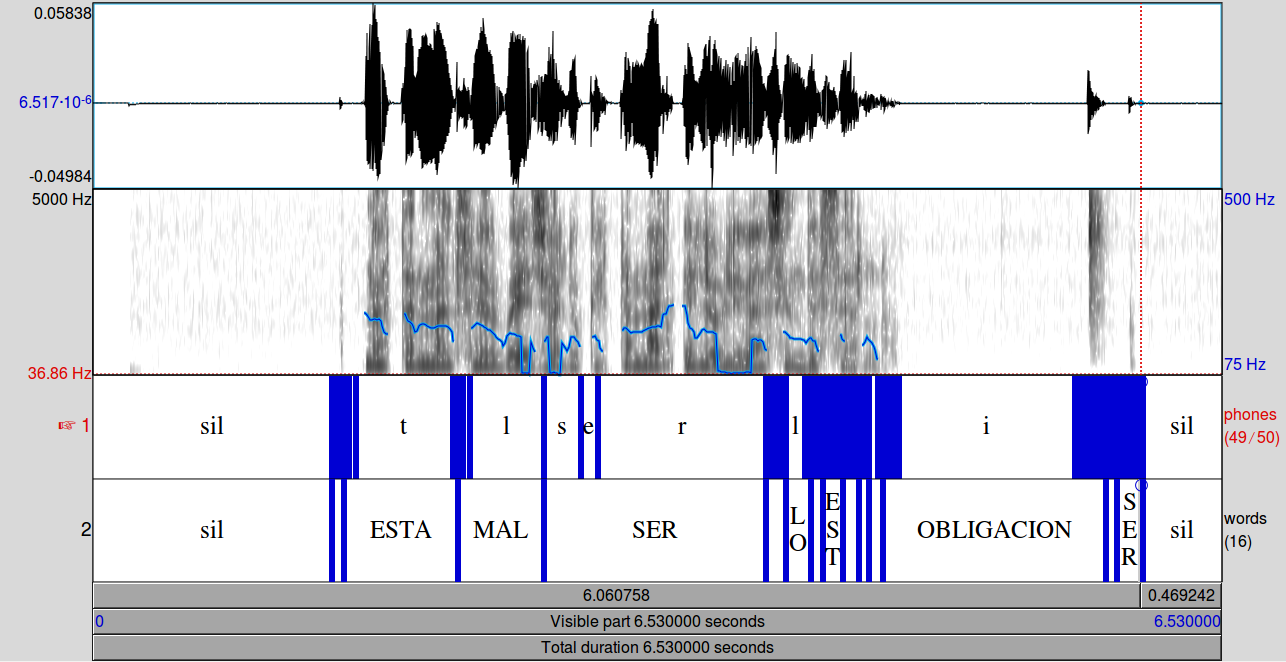
\includegraphics[width=0.8\textwidth]{alineacion_mala_inf} }
    \caption{Alineación mala}
\end{figure}


\subsection{Errores comunes}

Es muy importante descartar los audios mal alineados ya que sino cuando los procese el extractor nos darían información errónea. Fuimos chequeando cada audio y analizando si la alineación fue correcta. Para realizar esta tarea utilizamos el programa Praat. Los errores mas comunes fueron:
%todo citar bien a praat

\begin{itemize}
    \item \textbf{Ruido de fondo:} los casos donde el alineador se comporta de peor manera son los que se escuchan ruido de fondo. En esos casos las alineaciones resultan muy malas. Lamentablemente en nuestro caso esto es muy común. 

    \item \textbf{Mouse click al finalizar:} sucede que el ambiente donde los hablantes realizaban las grabaciones no estaba bien aislado. Pasó en muchas oportunidades que el click de finalizar del mouse se grabó como parte final de la grabación (Ver Fig. \ref{click_final}). Ese sonido se grabó y afectó la alineación de forma tal que se tomaba como habla.
    
\begin{figure}[h!]
    \centerline{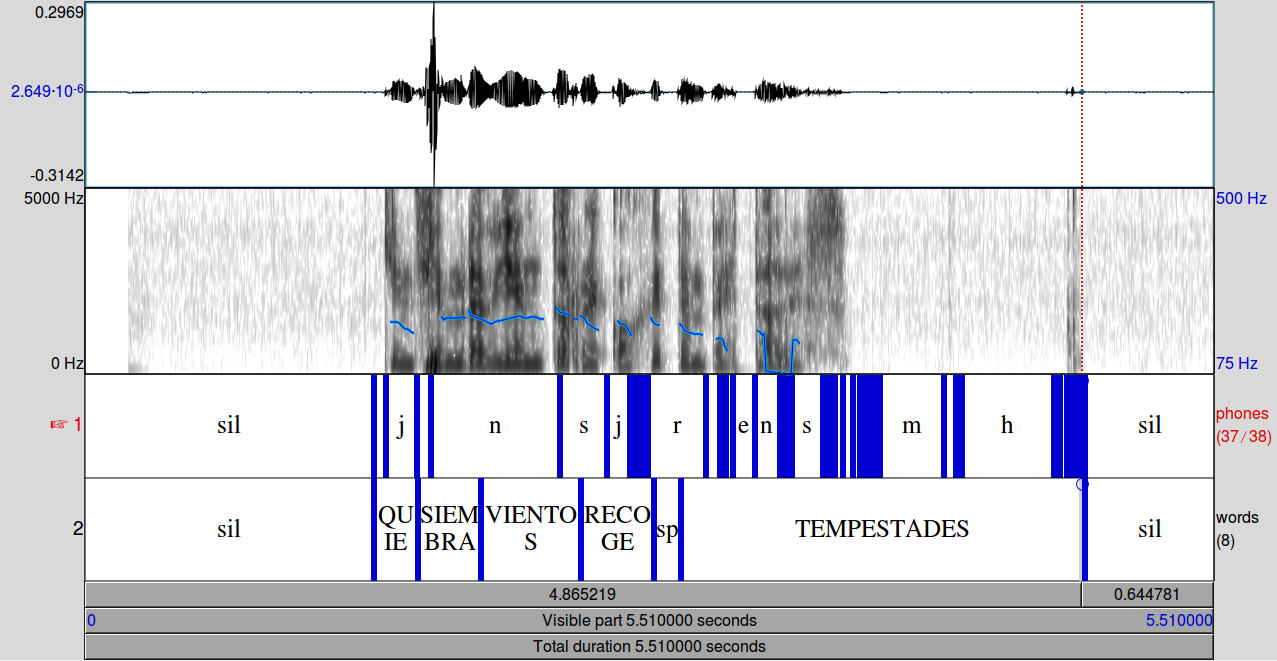
\includegraphics[width=0.8\textwidth]{click_al_final_inf} }
    \caption{Click al final}
    \label{click_final}
\end{figure}

    \item \textbf{Saturación del micrófono:} el volumen del micrófono es configurado por el hablante. Es por ello que debemos confiar en su buena voluntad. Sucede que muchas veces la grabación fue buena pero al final tuvo una entonación mas mucho mas fuerte que las demás, haciendo que posteriormente la alineación no sea precisa.

    \item \textbf{Estiramiento de la /s/ final:} en varias oportunidades se quiso exagerar la entonación. Las frases finalizadas en /s/ fueron grabadas en muchos casos sosteniendo ese fonema por tiempo prolongado. A pesar de que fue alineado correctamente en toda su duración, este fue llevado a una duración entendible. El problema que surgió en estos casos fue que el hablante no supo pronunciar la frase de la forma mas natural posible. Este fue el motivo por el cual se modificó.
\end{itemize}

\section{Corrección de errores}

Para corregir los errores descriptos debimos chequear cada uno de los textgrids. Los resultados de la cantidad de textgrid corregidos son:

\begin{table}[h]
\centering
\begin{tabular}{|l|c|c|c|c|}
\hline
\textbf{}  & \textbf{Bs.As. } & \textbf{Cba.} & \textbf{Total} \\ \hline
\textbf{Modificados}  & 101 & 88 & 189 \\ \hline
\textbf{Correctos sin modificación}  & 119 & 2 & 121 \\ \hline
\end{tabular}
\end{table}

%todo: leer bien el mail de prosodylab
Esta forma se realizó ya que eran pocos audios. Otro modo de hacer esto pero de forma automática puede ser de la siguiente forma. Cuando se realiza la alineación, se crea un archivo llamado .SCORES. Este archivo posee los valores de verosimilitud de cada alineación. Entonces este archivo podría servir para definir si un audio esta bien alineado. Si la alineación superó un umbral pre-configurado, el audio estará bien alineado y se podrá utilizar para el estudio, sino el audio se descartará. Vale aclarar que esto puede tener falsos positivos. Esta idea podría realizarse en trabajos futuros.

\chapter{Análisis}

En esta sección mostraremos los resultados que obtuvimos luego de realizar la extracción. Primero presentaremos el Baseline que consideramos. Luego describiremos el modelo de testing utilizando los datos recolectados. Explicaremos los clasificadores utilizados y en base a test estadísticos notaremos si aportan datos significativos. Por último, analizaremos los atributos más descriptivos de cada grupo.

\section{Baseline}

No hay ningún trabajo que trate de distinguir entre porteños y cordobéces a partir de su habla. Es por eso que el baseline se va a determinar a través del algoritmo mayority class.

Imaginemos que tenemos un algoritmo que siempre elige un mismo grupo, por ejemplo Buenos Aires. Este algoritmo utilizando nuestros datos tendría una performance buena. Al tener más hablantes de Buenos Aires que de Córdoba en nuestro set de datos acertaría más del 50\% de las veces. En nuestro caso tendrá (Completame XX)\% de efectividad. Este es el porcentaje a superar. 

%Pensemos que para determinar si una persona corresponde a alguno de los grupos vamos a tirar una moneda. Empíricamente podemos afirmar que en promedio la probabilidad de que salga algún grupo es 1/2. Gracias a la Ley de los Grandes Números podemos afirmar que, para valores grandes, esto va a tender a la Esperanza. Entonces, si nosotros queremos identificar un hablante utilizando el azar nos dará el 50\% de efetividad.

%Cabe aclarar que nuestro set de datos no esta debidamente balanceado. Tuvimos más grabaciones de Buenos Aires que de Córdoba. Es por eso que el entrenamiento también va a ser desbalanceado. Por este motivo puede suceder que al clasificar a un hablante en un test se obtenga mejores resultados para características de Buenos Aires que de Córdoba. Lamentablemente eso es una problemática de los datos obtenidos.

Cabe aclarar que si nuestro set de datos estuviera debidamente balanceado este porcentaje no sería tan alto. Lo ideal sería poder tener muestras balanceadas. Al tener este desbalance, puede suceder que al clasificar a un hablante en un test se obtenga mejores resultados para características de Buenos Aires que de Córdoba. Lamentablemente eso es una problemática de los datos obtenidos.

Utilizamos la herramienta de Machine Learning Weka para poder hacer el análisis. Esta nos provee un clasificador dummy descripto anteriormente. Este se llama ZeroR que es el algoritmo que siempre elige el mayor grupo.

\section{Modelo de testing}

La complejidad del problema y la forma en que fue realizado el experimento nos lleva a tener que descartar un modelo de testing común. Si utilizamos un modelo estándar deberíamos dividir los audios en 2 grupos, uno lo usaríamos para entrenar y otro para testear. Podría surgir el problema de que un hablante tenga audios en el conjunto de training y en el de testing. En ese caso el test sería erróneo ya que estaríamos entrenando con datos que luego serían testeados.

Para evitar este inconveniente debímos tomar en cuenta los hablantes a la hora de dividir los grupos. Vamos a dividir los grupos de train y test eligiendo al azar hablantes. Cuando tomemos un hablante al azar, debemos agregar todos sus audios grabados. En el siguiente pseudocódigo se explica la metodología. 

\lstset{ %
language=C++,                % choose the language of the code
basicstyle=\footnotesize,       % the size of the fonts that are used for the code
numbers=left,                   % where to put the line-numbers
numberstyle=\footnotesize,      % the size of the fonts that are used for the line-numbers
stepnumber=1,                   % the step between two line-numbers. If it is 1 each line will be numbered
numbersep=5pt,                  % how far the line-numbers are from the code
backgroundcolor=\color{white},  % choose the background color. You must add \usepackage{color}
showspaces=false,               % show spaces adding particular underscores
showstringspaces=false,         % underline spaces within strings
showtabs=false,                 % show tabs within strings adding particular underscores
frame=single,           % adds a frame around the code
tabsize=2,          % sets default tabsize to 2 spaces
captionpos=b,           % sets the caption-position to bottom
breaklines=true,        % sets automatic line breaking
breakatwhitespace=false,    % sets if automatic breaks should only happen at whitespace
escapeinside={\%*}{*)}          % if you want to add a comment within your code
}
\begin{lstlisting}
    Generador de Test:
    Input: conjunto audios
    Output: < conjunto train, conjunto test >
    train <- audios
    test <- {}
    mientras percentage < 0.1:
        hablante_BsAs <- Elegir al azar(audios)
        grabaciones_BsAs <- ObtenerGrabaciones(hablante_BsAs, audios)
    
        hablante_Cba <- Elegir al azar(audios)
        grabaciones_Cba <- ObtenerGrabaciones(hablante_Cba, audios)
    
        tests <- tests U grabaciones_BsAs U grabaciones_Cba
        train <- train - grabaciones_BsAs - grabaciones_Cba
    
        percentage <- Tam(test) / Tam(train) 
    
    Devolver <train, test>
\end{lstlisting}

Este proceso lo debemos realizar 10 veces para poder evitar que hayamos tenido suerte al generar el test. Luego de generado estos 10 pares de grupos de train y test vamos a utilizarlos para entrenar clasificadores.

\section{Clasificadores}

Vamos a entrenar varios clasificadores para poder determinar si el análisis de atributos que realizamos aporta mayor información a la hora de detectar un hablante. Los clasificadores propuestos son: 

\paragraph{Repeated Incremental Pruning to Produce Error Reduction (RIPPER) \cite{Cohen1995} - Implementación JRip:}

%http://weka.sourceforge.net/doc.dev/weka/classifiers/rules/JRip.html
%http://www.cs.utsa.edu/~bylander/cs6243/cohen95ripper.pdf
%https://indico.cern.ch/event/34666/session/13/material/slides/0?contribId=16 pag 21

Este algoritmo divide el conjunto de entrada en pequeños grupos. Para cada uno va generando reglas que lo describan de forma golosa incremental. Luego cuando no puede describir más a ese grupo lo extrae y sigue con otro. Cuando estos conjuntos superan una cierta dimensión el algoritmo se detiene. Este algoritmo sirve mucho para datos no balanceados.

\paragraph{C4.5 \cite{Quinlan1993} - Implementación J48:}

%http://en.wikipedia.org/wiki/C4.5_algorithm
%http://weka.sourceforge.net/doc.dev/weka/classifiers/trees/J48.html

Este algoritmo genera un árbol de decisión que es muy usado para clasificación. Dada una serie de muestras con varios atributos: Para cada atributo calcula la ganancia de información. Elige el que tenga mejor ganancia entre todos los atributos y con el crea un nodo en el árbol. Aplica recursivamente por cada rama. Si las muestras pertenecen a la misma clase o los atributos no proveen información se crea solo una hoja, este es el caso base.

\paragraph{Support Vector Machines \cite{Platt98sequentialminimal} - Implementación Function SMO:}

%http://en.wikipedia.org/wiki/Support_vector_machine
%http://machinelearning.wustl.edu/mlpapers/paper_files/BordesEWB05.pdf
%http://en.wikipedia.org/wiki/Sequential_minimal_optimization
%http://research.microsoft.com/pubs/69644/tr-98-14.pdf

Support vector machines es un problema por el cual se intenta separar muestras en dos clasificaciones distintas a traves de un hiperplano. Este hiperplano se construye utilizando los datos de entrada y sirve para clasificar las muestras en los dos grupos de forma óptima. Entonces utilizando este hiperplano, se puede etiquetar cada dato de entrada con su clasificación observando de que lado del hiperplano se encuentra.

\paragraph{Naive Bayes \cite{DBLP:conf/flairs/Zhang04} - Implementación homónima:}

%http://www.cs.unb.ca/profs/hzhang/publications/FLAIRS04ZhangH.pdf
%http://en.wikipedia.org/wiki/Naive_Bayes_classifier

Un clasificador de este tipo asume que cada atributo muestra una característica en particular de su clase pero no esta relacionado con otro atributo. Cada una de estos atributos contribuye de manera independiente a la clasificación de su clase. Utiliza fuertemente teorema de Bayes y que cada uno de los atributos es independiente. 

Más adelante describiremos los parámetros utilizados para cada uno.

\section{Tests estadísticos}

Vamos a utilizar los resultados de cada clasificador para ver si los resultados son significativamente relevantes. Los resultados que vamos a utilizar van a ser el vector resultante de los 10 grupos de tests utilizando el clasificador ZeroR contrastado con algún clasificador más sofisticado, por ejemplo: JRip, J48, Function SMO, NaiveBayes.
Para ello vamos a realizar dos principales tests: Wilcoxon signed-rank y Test de Student. 

\subsection{Wilcox Test}

Primero realizaremos Wilcox Test ya que necesita menos presunciones. Para realizar este test debemos cumplir que:

\begin{itemize}
    %Data are paired and come from the same population.
    \item Los datos son presentados de a pares y vienen de la misma población: esto sucede gracias a como armamos los tests. La población también siempre es la misma.
    %Each pair is chosen randomly and independently.
    \item Cada par es elegído al azar y independiente del resto: cada grupo generado para testing esta armado de forma azarosa ya que la elección de cada hablante se realiza de esta forma.
    %The data are measured at least on an ordinal scale, but need not be normal.
    \item Los datos estan medidos sobre una escala ordinal y no necesariamente debe provenir de una distribución Normal: esta característica es fundamental ya que no estamos seguros que nuestros datos provengan de una distribución Normal.
\end{itemize}

El input del mismo va a ser el vector resultante del test baseline ZeroR con el vector de los demás clasificadores. Las hipótesis van a ser:

\vspace{0.5cm}
\hspace{2cm}Ho: Clasificador alternativo no es mejor que ZeroR
\vspace{0.25cm}

\hspace{2cm}H1: Clasificador alternativo es mejor que ZeroR
\vspace{0.5cm}

donde Clasificador alternativo se refiere a los demás clasificadores. 
Cada uno de los tests nos va a dar un p-valor.
Si este es mayor 0,05 No hay evidencia suficiente para determinar que el clasificador alternativo es mejor.
Si de lo contrario, es menor Si podemos rechazar Ho y asegurar que el alternativo es mejor. 

Luego chequearemos si nuestra muestra es de distribución Normal. Si es ese el caso haremos el Test de Student. Para chequear Normalidad vamos a utilizar el test de Shapiro-Wilk.

\subsection{Análisis Shapiro-Wilk Test}

%todo: pensar si debo explicar todo el metodo o no hace falta
%http://es.wikipedia.org/wiki/Test_de_Shapiro%E2%80%93Wilk

%En estadística, el Test de Shapiro–Wilk se usa para contrastar la normalidad de un conjunto de datos. Se plantea como hipótesis nula que una muestra x1, ..., xn proviene de una población normalmente distribuida. Fue publicado en 1965 por Samuel Shapiro y Martin Wilk.1 Se considera uno de los test más potentes para el contraste de normalidad, sobre todo para muestras pequeñas (n<30).

El Test de Shapiro-Wilk lo utilizamos para notar la normalidad del conjunto de datos. Lo utilizamos ya que posee un buen desempeño en pequeñas muestras.

%Interpretación: Siendo la hipótesis nula que la población está distribuida normalmente, si el p-valor es menor a alfa (nivel de confianza) entonces la hipótesis nula es rechazada (se concluye que los datos no vienen de una distribución normal). Si el p-valor es mayor a alfa, no se rechaza la hipótesis y se concluye que los datos siguen una distribución normal.

Planteamos como hipótesis nula que la población esta distribuida de forma normal, aplicamos el estadístico de este test y si el p-valor nos da mayor a 0,05 entonces la hipótesis nula es rechazada. Si en cambio es menor a 0,05 no se puede rechazar Ho.

Este test se realiza individualmente para cada vector resultado. O sea, debemos chequear que los resultados de ZeroR para ver si su distribución se asemeja a la distribución Normal. Esto para cada resultado de los clasificadores. Si ambos tuvieron p-valor > 0,05, por ejemplo ZeroR y J48, se puede realizar el Student Test. 

\subsection{Student Test}

%En estadística, una prueba t de Student, prueba t-Student, o Test-T es cualquier prueba en la que el estadístico utilizado tiene una distribución t de Student si la hipótesis nula es cierta. Se aplica cuando la población estudiada sigue una distribución normal pero el tamaño muestral es demasiado pequeño como para que el estadístico en el que está basada la inferencia esté normalmente distribuido, utilizándose una estimación de la desviación típica en lugar del valor real. Es utilizado en análisis discriminante.

%A t-test is any statistical hypothesis test in which the test statistic follows a Student's t distribution if the null hypothesis is supported. It can be used to determine if two sets of data are significantly different from each other, and is most commonly applied when the test statistic would follow a normal distribution if the value of a scaling term in the test statistic were known. When the scaling term is unknown and is replaced by an estimate based on the data, the test statistic (under certain conditions) follows a Student's t distribution.

Para los vectores que poseen una distribución Normal vamos a aplicarle este test. Este nos provee una forma de determinar si dos conjuntos de test son significativa mente distintos. De la misma forma que planteamos la hipótesis de Wilcox test, este va a tener las mismas hipótesis. O sea: 

\vspace{0.5cm}
\hspace{2cm}Ho: Clasificador alternativo no es mejor que ZeroR
\vspace{0.25cm}

\hspace{2cm}H1: Clasificador alternativo es mejor que ZeroR
\vspace{0.5cm}

La ventaja de usarlo es que, al saber que distribución representa, vamos a ser mas precisos a la hora de calcular su p-valor. Aplicando el estadístico vamos a obtener un p-valor. De la misma forma, si este es mayor a 0,05 no hay evidencia suficiente para rechazar Ho. De lo contrario, si hay evidencia y rechazamos Ho.

\section{Resultados}

Todos tests fueron realizados utilizando R versión 3.0.1.

\subsection{Clasificadores}
%tabla de weka comparando cada uno de los clasificadores: ZeroR, JRIp, J48, FSMO, NaiveBayes
Los resultados para los distintos clasificadores fueron:

\begin{table}[H]
\centering
\begin{tabular}{|l|c|c|c|c|c|c|}
\hline
\textbf{}  & \textbf{ZeroR} & \textbf{JRip} & \textbf{J48} & \textbf{Function SMO} & \textbf{NaiveBayes} \\ \hline
\textbf{Test 1}  & 44.6809 & 57.4468 & 44.6809 & 55.3191 & 59.5745\\ \hline
\textbf{Test 2}  & 24.3243 & 45.9459 & 24.3243 & 51.3514 & 40.5405\\ \hline
\textbf{Test 3}  & 32.1429 & 46.4286 & 32.1429 & 46.4286 & 64.2857\\ \hline
\textbf{Test 4}  & 48.8889 & 46.6667 & 48.8889 & 62.2222 & 57.7778\\ \hline
\textbf{Test 5}  & 30.303 & 39.3939 & 30.303 & 45.4545 & 63.6364\\ \hline
\textbf{Test 6}  & 46.3415 & 53.6585 & 46.3415 & 68.2927 & 68.2927\\ \hline
\textbf{Test 7}  & 38.7097 & 38.7097 & 25.8065 & 45.1613 & 58.0645\\ \hline
\textbf{Test 8}  & 30.303 & 39.3939 & 30.303 & 45.4545 & 63.6364\\ \hline
\textbf{Test 9}  & 30.303 & 39.3939 & 30.303 & 45.4545 & 63.6364\\ \hline
\textbf{Test 10} & 37.2881 & 42.3729 & 37.2881 & 49.1525 & 54.2373\\ \hline
\end{tabular}
\end{table}

donde Test 1 corresponde al primer par < conjunto train, conjunto test > y así sucesivamente.

\subsection{Wilcox y Student Test}

Vamos a mostrar los resultados de estos tests estadísticos.

\begin{table}[H]
\centering
\begin{tabular}{|l|c|c|c|c|c|c|}
\hline
\textbf{}  & \textbf{Student Test} & \textbf{Wilcox Test} \\ \hline
\textbf{ZeroR y JRip}  & 0.001644 & 0.006269 \\ \hline
\textbf{ZeroR y J48}  & 0.8283 & 0.9772 \\ \hline
\textbf{ZeroR y NaiveBayes}  & 1.225e-05 & 0.002897 \\ \hline
\textbf{ZeroR y Function SMO}  & 8.266e-06 & 0.002897 \\ \hline
\end{tabular}
\end{table}

\section{Selección de atributos de forma automática}

En esta sección se aplicará a los distintos atributos evaluadores para analizar cual posee mayor importancia. Los evaluadores utilizados son InfoGain y ClassifierSubsetEvaluator. 

\subsection*{Attribute Evaluator: InfoGain}
%http://weka.sourceforge.net/doc.dev/weka/attributeSelection/InfoGainAttributeEval.html

\paragraph*{Utilizando todos los atributos}

\begin{table}[H]
\centering
\begin{tabular}{|c|l|c|c|c|c|c|}
\hline
 0.07231     & FON\_consonant\_norm \\ \hline
 0.07217     & FON\_vowel\_norm \\ \hline
 0.03963     & \textbf{SIL\_syllableAccent\_normhd} \\ \hline
 0.03963     & \textbf{SIL\_prevSyllableAccent\_normhd }\\ \hline
 0.02332     & FON\_ll\_norm \\ \hline
 0.02285     & FON\_Sfinal\_norm \\ \hline
 0.02226     & ACU\_MinLL\_1 \\ \hline
 0.02144     & ACU\_AverageLL\_1 \\ \hline
 
\end{tabular}
\end{table}

\paragraph*{Utilizando solo los atributos sobre fonemas}

\begin{table}[H]
\centering
\begin{tabular}{|c|l|c|c|c|c|c|}
\hline
 0.07231     & FON\_consonant\_norm \\ \hline
 0.07217     & FON\_vowel\_norm \\ \hline
 0.02332     & FON\_ll\_norm \\ \hline
 0.02285     & FON\_Sfinal\_norm \\ \hline
 0.00857     & FON\_ll\_normhd  \\ \hline
\end{tabular}
\end{table}

\paragraph*{Utilizando solo los atributos silábicos}

\begin{table}[H]
\centering
\begin{tabular}{|c|l|c|c|c|c|c|}
\hline
 0.03963     & SIL\_syllableAccent\_normhd \\ \hline
 0.03963     & SIL\_prevSyllableAccent\_normhd \\ \hline
 0           & SIL\_prevSyllableAccent\_norm \\ \hline
 0           & SIL\_syllableAccent\_norm \\ \hline
\end{tabular}
\end{table}

\paragraph*{Utilizando solo los atributos acústicos}

\begin{table}[H]
\centering
\begin{tabular}{|c|l|c|c|c|c|c|}
\hline
 0.02226     & ACU\_MinLL\_1  \\ \hline
 0.02144     & ACU\_AverageLL\_1  \\ \hline
 0.01438     & ACU\_MaxLL\_5  \\ \hline
 0.01232     & ACU\_MaxKT\_15  \\ \hline
 0.01219     & ACU\_MaxLL\_6  \\ \hline
\end{tabular}
\end{table}

\subsection*{Attribute Evaluator: ClassifierSubsetEvaluator}

\begin{table}[H]
\centering
\begin{tabular}{|l|c|c|c|c|c|c|}
\hline
ACU\_AverageRR\_0 \\ \hline
ACU\_MaxKT\_11 \\ \hline
ACU\_MaxSC\_7 \\ \hline
ACU\_MinKT\_0 \\ \hline
ACU\_MinLL\_1 \\ \hline
ACU\_MinSC\_22 \\ \hline
FON\_Sfinal\_normhd \\ \hline
FON\_vowel\_normhd \\ \hline
 
\end{tabular}
\end{table}

\section{Combinando clases de atributos}

Combinando los tipos de atributos definidos se puede apreciar cuanto aporta cada clase de los mismos. Vamos a agregar los tipos de atributos y vamos a analizar como se incrementa el porcentaje de exactitud para la clasificación. El conjunto de datos utilizado es el \textit{test0} y se utiliza \textit{JRip} como clasificador.

%poner tabla: FON, SIL, ACU y sus combinaciones para clasificacion 
\begin{table}[H]
\centering
\begin{tabular}{|l|c|c|}
\hline
\textbf{}  & \textbf{Porcentaje  JRip}  & \textbf{Porcentaje  NaiveBayes}   \\ \hline
Baseline & 44.6809 & 44.6809 \\ \hline
SIL & 42.5532 & 53.1915 \\ \hline
FON & 55.3191 & 57.4468 \\ \hline
ACU & 55.3191 & 59.5745 \\ \hline
SIL + FON & 42.5532 & 57.4468 \\ \hline
FON + ACU & 53.1915 & 61.7021 \\ \hline
SIL + ACU & 57.4468 &  61.7021 \\ \hline
SIL + FON + ACU & 57.4468 & 59.5745 \\ \hline
\end{tabular}
\end{table}

Lo esperable es que aumentando los atributos se aumenta el porcentaje de clasificación. A grandes rasgos, aquí sucede pero dejando de lado el conjunto de atrbutos acústicos. Al agregar este conjunto la performance baja notablemente. Creemos que esto sucede por los distintos ambientes de grabación de cada hablante. Estos aportan mucho ruido y por ello no se puede extraer información útil para la clasificación.

\chapter{Conclusiones}
\chapter{Trabajos futuros}

Algunos trabajos futuros que se desprenden de este trabajo son:

\paragraph*{Filtro por ruido con SoX:} Se podría analizar mejor los audios si se le aplicara algún filtro que extraiga el ruido. De esta forma se podría mejorar los atributos acústicos. 

\paragraph*{Chequeador cruzado con grabación:} Que no se muestre la frase a decir, sino que se escuche un audio y se tenga repetirlo. Este audio es el de un hablante anterior pero que se le aplicó un filtro para evitar exponer su acento. De esta forma, chequeamos que se diga lo que se quiere decir y nos aseguramos espontaneidad.

\paragraph*{Chequeador cruzado:} Que el hablante diga si una grabación de un hablante anterior dijo lo que tenía que decir, o se equivocó. En este caso, serviría mucho para chequear los datos. 

\paragraph*{Validación de calidad de sonido:} Cuando un hablante graba un audio este debe pasar una validación en el servidor para poder continuar con el siguiente. Sino fue satisfactorio, se pude grabar devuelta. Evitaría el ruido generado por el ambiente. 

\paragraph*{Clasificación en vivo:} Realizar la clasificación al agregar un hablante nuevo. De esta forma, se puede darle una respuesta a que grupo pertenece. Revalidar el modelo al agregarse un nuevo Hablante. 

\chapter{Apéndice: marcas prosódicas}

En la figura \ref{tab:myfirstlongtable} podemos ver las marcas prosódicas de cada frase.

\centering
\begin{longtable}{| p{0.3\textwidth} | p{0.6\textwidth} |} 
\hline
\textbf{Frase}  & \textbf{Prosodia}  \\ \hline

'no hay dos sin tres' & [['no'], ['aj'], ['dos*'], ['sin'], ['tres*']] \\ \hline
'mas dificil que encontrar una aguja en un pajar' & [['mas'], ['di', 'fi*', 'sil'], ['ke'], ['eN', 'kon', 'trar*'], ['una'], ['a', 'Gu*', 'xa'], ['en'], ['un'], ['pa', 'xar*']] \\ \hline
'mas perdido que turco en la neblina' & [['mas'], ['per', 'Di*', 'Do'], ['ke'], ['tur*', 'ko'], ['en'], ['la'], ['ne', 'Bli*', 'na']] \\ \hline
'no le busques la quinta pata al gato' & [['no'], ['le'], ['buh*', 'kes'], ['la'], ['kin*', 'ta'], ['pa*', 'ta'], ['al'], ['ga*', 'to']] \\ \hline
'todo bicho que camina va al asador' & [['to', 'do'], ['bi*', 'cho'], ['ke'], ['ka', 'mi*', 'na'], ['va'], ['al'], ['a','sa','dor*']] \\ \hline
'caminante no hay camino se hace camino al andar' & [['ka', 'mi', 'nan*', 'te'], ['no'], ['aj'], ['ka', 'mi*', 'no'], ['se'], ['ha*', 'ce'], ['ka', 'mi*', 'no'], ['al'], ['an', 'dar*']] \\ \hline
'se te escapo la tortuga' & [['se'], ['te'], ['eh', 'ka', 'po*'], ['la'], ['tor', 'tu*', 'Ga']] \\ \hline
'todos los caminos conducen a roma' & [['to', 'Dos'], ['los'], ['ka', 'mi*', 'nos'], ['kon', 'du*', 'cen'], ['a'], ['Ro*', 'ma']] \\ \hline
'no hay mal que dure cien anos' & [['no'], ['aj'], ['mal*'], ['ke'], ['du*', 're'], ['cien*'], ['a*', 'nos']] \\ \hline
'siempre que llovio paro' & [['sjem*', 'pre'], ['ke'], ['Zo', 'Bjo*'], ['pa', 'ro*']] \\ \hline
'cria cuervos que te sacaran los ojos' & [['krj*', 'a'], ['kwer*', 'Bos'], ['ke'], ['te'], ['sa', 'ka', 'ran*'], ['los'], ['o*', 'xos']] \\ \hline
'la tercera es la vencida' & [['la'], ['ter', 'se*', 'ra'], ['es'], ['la'], ['ben', 'si*', 'Da']] \\ \hline
'calavera no chilla' & [['ka', 'la', 'Be*', 'ra'], ['no'], ['Hi*', 'Za']] \\ \hline
'la gota que rebalso el vaso' & [['la'], ['go*', 'ta'], ['ke'], ['Re', 'Bal', 'so*'], ['el'], ['ba*', 'so']] \\ \hline
'la suegra y el doctor cuanto mas lejos mejor' & [['la'], ['swe*', 'Gra'], ['y'], ['el'], ['dok', 'tor*'], ['kwan', 'to'], ['mas'], ['le*', 'xos'], ['me', 'xor*']] \\ \hline
'a la mujer picaresca cualquiera la pesca' & [['a'], ['la'], ['mu', 'Cer*'], ['pi','ka', 'reh*','ka'], ['kwal', 'kje*', 'ra'], ['la'], ['peh*', 'ka']] \\ \hline
'quien siembra vientos recoge tempestades' & [['kj*', 'en'], ['sjem*', 'bra'], ['bjen*', 'tos'], ['Re', 'ko*', 'Ce'], ['tem', 'peh', 'ta*', 'Des']] \\ \hline
'un grano no hace granero pero ayuda a su companero' & [['un'], ['gra*', 'no'], ['no'], ['ha*', 'ce'], ['gra', 'ne*', 'ro'], ['pe', 'ro'], ['a', 'yu*', 'da'], ['a'], ['su'], ['com', 'pa', 'ne*', 'ro']] \\ \hline
'la arquitectura es el arte de organizar el espacio' & [['la'], ['ar', 'ki', 'tek', 'tu*','ra'], ['es'], ['el'], ['ar*', 'te'], ['de'], ['or', 'Ga', 'ni', 'sar*'], ['el'], ['eh', 'pa*', 'sjo']] \\ \hline
'el amor actua con el corazon y no con la cabeza' & [['el'], ['a', 'mor*'], ['ak', 'tw*', 'a'], ['kon'], ['el'], ['ko', 'ra', 'son*'], ['i'], ['no'], ['kon'], ['la'], ['ka','Be*', 'sa']] \\ \hline
'no dudes actua' & [['no'], ['du*', 'Des'], ['ak', 'tw*', 'a']] \\ \hline
'el nino es realista el muchacho idealista el hombre esceptico y el viejo mistico' & [['el'], ['ni*', 'no'], ['es'], ['re', 'a', 'lis*', 'ta'], ['el'], ['mu', 'cha*', 'cho'], ['i','de', 'a', 'lis*', 'ta'], ['el'], ['hom*', 'bre'], ['es', 'cep*', 'ti', 'co'], ['y'], ['el'], ['vie*', 'jo'], ['mis*', 'ti', 'co']] \\ \hline
'perro que ladra no muerde' & [['pe*', 'Ro'], ['ke'], ['la*', 'Dra'], ['no'], ['mwer*', 'De']] \\ \hline
'la musica es sinonimo de libertad de tocar lo que quieras y como quieras' & [['la'], ['mu*','si','ka'], ['es'], ['si', 'no*', 'ni', 'mo'], ['de'], ['li','Ber','taD*'], ['de'], ['to', 'kar*'], ['lo'], ['ke'], ['kje*','ras'], ['i'], ['ko','mo'], ['kje*','ras']] \\ \hline
'la belleza que atrae rara vez coincide con la belleza que enamora' & [['la'], ['be','Ze*','sa'], ['ke'], ['a', 'tra*', 'e'], ['Ra*', 'ra'], ['Bes*'], ['kojn', 'si*', 'De'], ['kon'], ['la'], ['be','Ze*','sa'], ['ke'], ['e','na','mo*','ra']] \\ \hline
'no esta mal ser bella lo que esta mal es la obligacion de serlo' & [['no'], ['eh', 'ta*'], ['mal*'], ['ser'], ['be*', 'Za'], ['lo'], ['ke'], ['eh', 'ta*'], ['mal*'], ['es'], ['la'], ['o', 'Bli','Ga', 'sjon*'], ['de'], ['ser*', 'lo']] \\ \hline
'la batalla mas dificil la tengo todos los dias conmigo mismo' & [['la'], ['ba', 'ta*', 'Za'], ['mas'], ['di','fi*','sil'], ['la'], ['teN*', 'go'], ['to','Dos'], ['los'], ['dj*', 'as'], ['kon', 'mi*', 'Go'], ['mis*', 'mo']] \\ \hline
'el que no llora no mama' & [['el'], ['ke'], ['no'], ['Zo*', 'ra'], ['no'], ['ma*', 'ma']] \\ \hline
'en la pelea se conoce al soldado solo en la victoria se conoce al caballero' & [['en'], ['la'], ['pe', 'le*', 'a'], ['se'], ['ko', 'no*', 'se'], ['al'], ['sol', 'da*', 'Do'], ['so*', 'lo'], ['en'], ['la'], ['bik', 'to*', 'rja'], ['se'], ['ko', 'no*', 'se'], ['al'], ['ka', 'Ba', 'Ze*', 'ro']] \\ \hline
'la lectura es a la mente lo que el ejercicio al cuerpo' & [['la'], ['lek', 'tu*', 'ra'], ['es'], ['a'], ['la'], ['men*', 'te'], ['lo'], ['ke'], ['el'], ['e', 'Cer', 'si*', 'sjo'], ['al'], ['kwer*', 'po']] \\ \hline
'el pez por la boca muere' & [['el'], ['pes*'], ['por'], ['la'], ['bo*', 'ka'], ['mwe*', 're']] \\ \hline
'el canape salio espectacular' & [['el'], ['ka', 'na', 'pe*'], ['sa', 'ljo*'], ['eh', 'pek', 'ta', 'ku', 'lar*']] \\ \hline
'el canape salio delicioso' & [['el'], ['ka', 'na', 'pe*'], ['sa', 'ljo*'], ['de', 'li', 'sjo*', 'so']] \\ \hline
'el canape salio riquisimo' & [['el'], ['ka', 'na', 'pe*'], ['sa', 'ljo*'], ['Ri', 'ki*', 'si', 'mo']] \\ \hline
'el repollo salio espectacular' & [['el'], ['Re', 'po*', 'Zo'], ['sa', 'ljo*'], ['eh', 'pek', 'ta', 'ku', 'lar*']] \\ \hline
'el repollo salio delicioso' & [['el'], ['Re', 'po*', 'Zo'], ['sa', 'ljo*'], ['de', 'li', 'sjo*', 'so']] \\ \hline
'el repollo salio riquisimo' & [['el'], ['Re', 'po*', 'Zo'], ['sa', 'ljo*'], ['Ri', 'ki*', 'si', 'mo']] \\ \hline
'el esparrago salio espectacular' & [['el'], ['eh', 'pa*', 'Ra', 'Go'], ['sa', 'ljo*'], ['eh', 'pek', 'ta', 'ku', 'lar*']] \\ \hline
'el esparrago salio delicioso' & [['el'], ['eh', 'pa*', 'Ra', 'Go'], ['sa', 'ljo*'], ['de', 'li', 'sjo*', 'so']] \\ \hline
'el esparrago salio riquisimo' & [['el'], ['eh', 'pa*', 'Ra', 'Go'], ['sa', 'ljo*'], ['Ri', 'ki*', 'si', 'mo']] \\ \hline
'en boca cerrada no entran moscas' & [['en'], ['bo*', 'ka'], ['se', 'Ra*', 'Da'], ['no'], ['en*', 'tran'], ['moh*', 'kas']] \\ \hline
'mas vale pajaro en mano que cien volando' & [['mas'], ['ba*', 'le'], ['pa*', 'xa', 'ro'], ['en'], ['ma*', 'no'], ['ke'], ['sjen*'], ['bo', 'lan*', 'do']] \\ \hline
'la curiosidad mato al gato' & [['la'], ['ku', 'rjo','si', 'DaD*'], ['ma', 'to*'], ['al'], ['ga*', 'to']] \\ \hline
'rio revuelto ganancia de pescadores' & [['Rj*', 'o'], ['Re', 'Bwel*', 'to'], ['ga', 'nan*', 'sja'], ['de'], ['peh', 'ka', 'Do*', 'res']] \\ \hline
'no hay que pedirle peras al olmo' & [['no'], ['aj'], ['ke'], ['pe', 'Dir*', 'le'], ['pe*', 'ras'], ['al'], ['ol*','mo']] \\ \hline

\caption{Marcas prosódicas} 
\label{tab:myfirstlongtable}
\end{longtable}

%%%% BIBLIOGRAFIA
\backmatter
\bibliography{ref}
\bibliographystyle{plain}
 
\end{document}
